%!LW recipe=latexmk-xelatex
\documentclass[compress]{beamer}

\usetheme[block=fill]{metropolis}

\usepackage{graphicx} % Allows including images
\usepackage{amsmath,amsfonts,amsthm,amssymb}
\usepackage{color}
\usepackage{xcolor,cancel}
\usepackage{tcolorbox}
\setbeamercolor{colorBoxStuff}{fg=black, bg=gray!30!white}
%\setitemize{label=\usebeamerfont*{itemize item}%
%	\usebeamercolor[fg]{itemize item}
%	\usebeamertemplate{itemize item}}
\definecolor{mDarkBrown}{HTML}{604c38}
\definecolor{mDarkTeal}{HTML}{23373b}
\definecolor{mLightBrown}{HTML}{EB811B}
\definecolor{mMediumBrown}{HTML}{C87A2F}
\definecolor{mygreen}{HTML}{98C2B9}
\definecolor{myyellow}{HTML}{DFD79C}
\definecolor{myblue}{HTML}{8CA7CC}
\definecolor{kern}{HTML}{8CC2B7}


\usepackage{float}
\usepackage{framed}
\usepackage{epsfig}
\usepackage{graphicx}
\usepackage{subcaption}
\usepackage{ulem}
\usepackage{hhline}
\usepackage{multirow}
\usepackage{comment}   
\usepackage{bbm}
\usepackage{tikz}   
\def\Put(#1,#2)#3{\leavevmode\makebox(0,0){\put(#1,#2){#3}}}
\newcommand*\mystrut[1]{\vrule width0pt height0pt depth#1\relax}
\newcommand{\eqdef}{\mathbin{\stackrel{\rm def}{=}}}


\newcommand{\bs}[1]{\boldsymbol{#1}}
\newcommand{\bv}[1]{\mathbf{#1}}
\newcommand{\R}{\mathbb{R}}
\newcommand{\E}{\mathbb{E}}

\DeclareMathOperator*{\argmin}{arg\,min}
\DeclareMathOperator*{\argmax}{arg\,max}
\DeclareMathOperator{\nnz}{nnz}
\DeclareMathOperator{\vol}{vol}
\DeclareMathOperator{\diag}{diag}
\DeclareMathOperator{\Var}{Var}
\DeclareMathOperator{\sinc}{sinc}
\DeclareMathOperator{\sign}{sign}
\DeclareMathOperator{\dist}{dist}
\DeclareMathOperator{\mv}{mv}
\DeclareMathOperator{\sgn}{sgn}
\DeclareMathOperator{\step}{step}
\DeclareMathOperator{\gap}{gap}
\DeclareMathOperator{\poly}{poly}
\DeclareMathOperator{\tr}{tr}
\DeclareMathOperator{\orth}{orth}
\newcommand{\norm}[1]{\|#1\|}
\captionsetup[subfigure]{labelformat=empty}
\captionsetup[figure]{labelformat=empty}
\DeclareMathOperator*{\lmin}{\lambda_{min}}
\DeclareMathOperator*{\lmax}{\lambda_{max}}

\newcommand{\specialcell}[2][c]{%
  \begin{tabular}[#1]{@{}c@{}}#2\end{tabular}}
\newcommand{\specialcellleft}[2][c]{%
\begin{tabular}[#1]{@{}l@{}}#2\end{tabular}
}

\newtheorem{claim}[theorem]{Claim}
%\newtheorem{corollary}[theorem]{Corollary}

\usepackage{tabstackengine}
\stackMath


%----------------------------------------------------------------------------------------
%	TITLE PAGE
%----------------------------------------------------------------------------------------

\title{CS-GY 6763: Lecture 13 \\ Fast Johnson-Lindenstrauss Transform, Sparse Recovery and Compressed Sensing}
\author{NYU Tandon School of Engineering, Prof. Christopher Musco}
\date{}

\begin{document}

\begin{frame}
	\titlepage 
\end{frame}

\metroset{titleformat=smallcaps}

\begin{frame}[t]
	\frametitle{randomized numerical linear algebra}
	\textbf{Main idea}: Speed up classical linear algebra problems using randomization.
	\begin{center}
		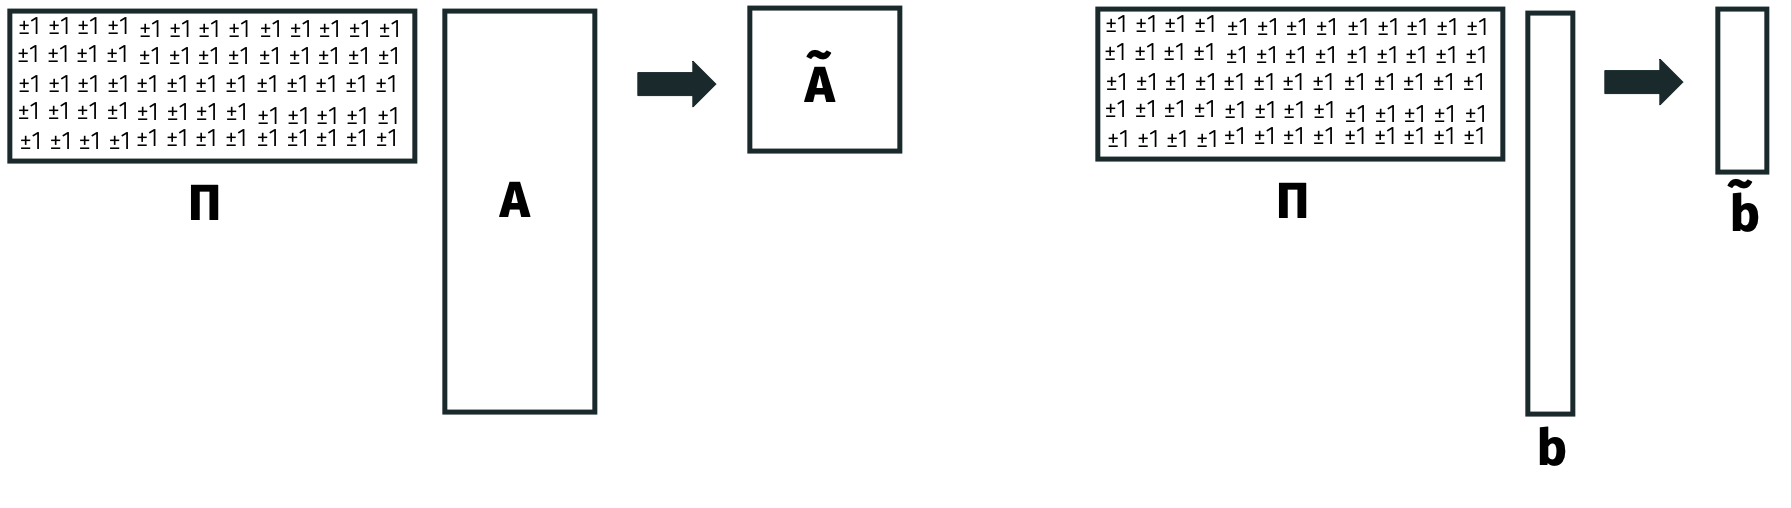
\includegraphics[width=.8\textwidth]{jlRegression.png}
	\end{center}
\vspace{-1em}
	\textbf{Input}: $\bv{A} \in \R^{n\times d}$, $\bv{b} \in \R^{n}$. 
	
	\textbf{Algorithm}: Let $\tilde{\bv{x}}^* = \argmin_{\bv{x}} \|\bs{\Pi}\bv{A}\bv{x} - \bs{\Pi}\bv{b}\|_2^2$.
	
	\textbf{Goal}: Want $\|\bv{A}\tilde{\bv{x}}^* - \bv{b}\|_2^2 \leq (1+\epsilon) \min_{\bv{x}} \|\bv{A}\bv{x} - \bv{b}\|_2^2$
\end{frame}


\begin{frame}[t]
	\frametitle{randomized numerical linear algebra}
	\begin{theorem}[Example: Randomized Linear Regression]
		Let $\bs{\Pi}$ be a properly scaled JL matrix (random Gaussian, sign, sparse random, etc.) with $m = O\left(\frac{d}{\epsilon^2}\right)$ rows. Then with probability $9/10$, for any $\bv{A}\in \R^{n\times d}$ and $\bv{b}\in \R^n$,
		\begin{align*}
			\|\bv{A}\tilde{\bv{x}} - \bv{b}\|_2^2 \leq (1+\epsilon) \|\bv{A}\bv{x}^* - \bv{b}\|_2^2
		\end{align*}
		where $\tilde{\bv{x}} = \argmin_{\bv{x}} \|\bs{\Pi}\bv{A}\bv{x} - \bs{\Pi}\bv{b}\|_2^2$.
	\end{theorem}
	Reduce from a $O(nd^2)$ time computation to an $O(d^3)$ time problem.
	\end{frame}

	\begin{frame}
	\frametitle{randomized numerical linear algebra}
	\begin{theorem}[Second Example: Randomized Low-Rank Approximation\footnote{See e.g. Sarlos, 2006 or Halko, Martinson, Tropp, 2011.}]
		Let $\bs{\Pi}$ be a properly scaled JL matrix (random Gaussian, sign, sparse random, etc.) with $m = O\left(\frac{k}{\epsilon}\right)$ rows. Then with probability $9/10$, for any $\bv{A}\in \R^{n\times d}$,
		\begin{align*}
			\|\bv{A} - \bv{A}\tilde{\bv{V}}_k\tilde{\bv{V}}_k^T\|_2^2 \leq (1+\epsilon) \|\bv{A} - \bv{A}_k\|_2^2
		\end{align*}
		where $\tilde{\bv{V}}_k$ contains the top $k$ right singular vectors of $\tilde{\bv{A}}$.
	\end{theorem}
	Reduce from a $O(ndk)$ time computation to an $O(dk^2)$ time problem.
	\end{frame}
	
	
	
	\begin{frame}
		\frametitle{subspace embeddings}
		\textbf{Key Ingredient:} 
		\begin{theorem}[Subspace Embedding JL]
			Let $\mathcal{U} \subset \R^n$ be a $d$-dimensional linear subspace in $\R^n$. If $\bs{\Pi}\in \R^{m\times d}$ is chosen from any distribution $\mathcal{D}$ satisfying the Distributional  JL Lemma, then with probability $1-\delta$,
			\begin{align*}
				(1-\epsilon)\|\bv{v}\|_2^2 \leq \|\Pi \bv{v}\|_2^2 \leq	(1+\epsilon)\|\bv{v}\|_2^2
			\end{align*}
			for \emph{all} $\bv{v} \in \mathcal{U}$, as long as  $m = O\left(\frac{d\log(1/\epsilon) + \log(1/\delta)}{\epsilon^2}\right)$.
		\end{theorem}
		\begin{center}
			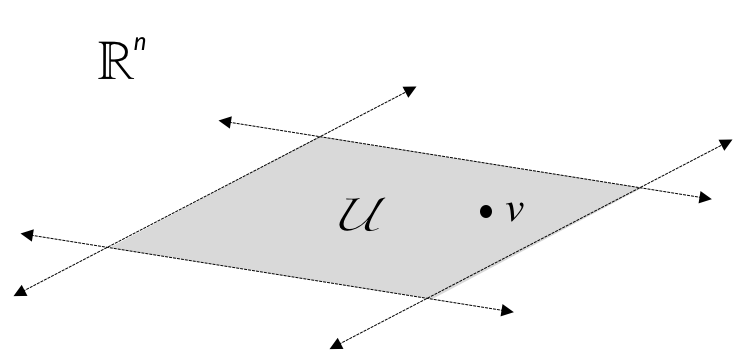
\includegraphics[width=0.4\textwidth]{subspace_vis.png}
		\end{center}
	\end{frame}
	
	
	\begin{frame}
		\frametitle{subspace embedding proof}
		\textbf{Proof idea:} Construct $\epsilon$-net, $N_\epsilon$, for the unit sphere, ${S}$. 
		\begin{enumerate}
			\item Prove that $\|\bs{\Pi}\bv{w}\|_2^2 = (1\pm \epsilon)\|\bv{w}\|_2^2$ for all $\bv{w}\in N_\epsilon$ using union bound.
			\item Use a direct argument to extend to the rest of sphere. 
		\end{enumerate}
		\vspace{-1em}
		\begin{center}
			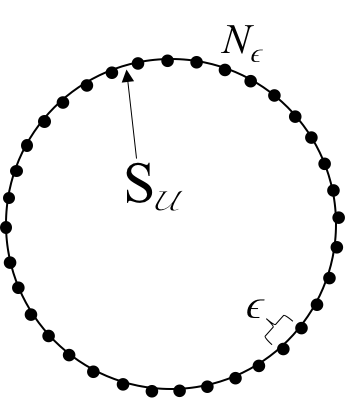
\includegraphics[width=0.3\textwidth]{2dnet.png}
		\end{center}
	\end{frame}
	
	\begin{frame}[t]
		\frametitle{$\epsilon$-net for the sphere}
		\begin{lemma}[$\epsilon$-net for the sphere]
			Let ${S}$ be a $d$ dimensional union sphere.
			For any $\epsilon \leq 1$, there exists a set $N_{\epsilon} \subset S$ with $| N_\epsilon | = \left(\frac{3}{\epsilon}\right)^d$ such that $\forall \bv{v} \in S$,
			\begin{align*}
				\min_{\bv{w} \in N_\epsilon} \|\bv{v} - \bv{w}\|_2 \leq \epsilon. 
			\end{align*}
		\end{lemma} 
	\begin{center}
		\textbf{We skipped the proof of this last time.}

		We will prove it using a common technique known as a ``volume'' argument.
	\end{center}
	\end{frame}

	\begin{frame}[t]
		\frametitle{$\epsilon$-net for the sphere}
		\begin{lemma}[$\epsilon$-net for the sphere]
			Let ${S}$ be a $d$ dimensional union sphere.
			For any $\epsilon \leq 1$, there exists a set $N_{\epsilon} \subset S$ with $| N_\epsilon | = \left(\frac{3}{\epsilon}\right)^d$ such that $\forall \bv{v} \in S$,
			\begin{align*}
				\min_{\bv{w} \in N_\epsilon} \|\bv{v} - \bv{w}\|_2 \leq \epsilon. 
			\end{align*}
		\end{lemma} 
		
		\textbf{Imaginary algorithm for constructing $N_\epsilon$}:
		\begin{itemize}
			\item Set $N_\epsilon = \{\}$
			\item While such a point exists, choose an arbitrary point $\bv{v} \in S$ where there is no $\bv{w} \in N_\epsilon$ with $\|\bv{v} - \bv{w}\| \leq \epsilon$. 
			\item Add $\bv{v}$ to $N_\epsilon$.
		\end{itemize}
		After running this procedure, we have $N_\epsilon = \{\bv{w}_1, \ldots, \bv{w}_{|N_\epsilon|}\}$ and $\min_{\bv{w} \in N_\epsilon} \|\bv{v} - \bv{w}\| \leq \epsilon$ for all $\bv{v} \in S$ as desired.
	\end{frame}
	
	\begin{frame}[t]
		\frametitle{$\epsilon$-net for the sphere}
		\begin{center}
			\textbf{\alert{How many steps does this procedure take?}}
			
			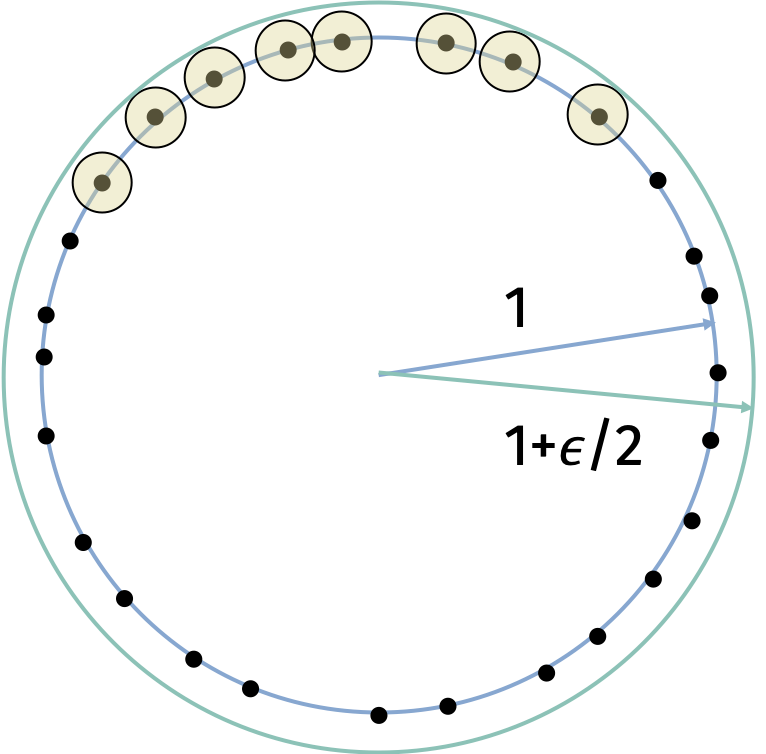
\includegraphics[width=.4\textwidth]{net_argument.png}
		\end{center}
	
		
		Can place a ball of radius $\epsilon/2$ around each $\bv{w}_i$ without intersecting any other balls. All of these balls live in a ball of radius $1+\epsilon/2$.
	\end{frame}
	
	\begin{frame}[t]
		\frametitle{$\epsilon$-net for the sphere}
		Volume of $d$ dimensional ball of radius $r$ is 
		\begin{align*}
			\vol(d,r) = c\cdot r^d,
		\end{align*}
		where $c$ is a constant that depends on $d$, but not $r$.
		\vspace{1em}
		From previous slide we have:
		\begin{align*}
			\vol(d,\epsilon/2) \cdot |N_\epsilon| &\leq \vol(d,1+\epsilon/2) \\  
			|N_\epsilon| &\leq \frac{\vol(d,1+\epsilon/2)}{\vol(d,\epsilon/2)} \\
			&\leq \left(\frac{1+\epsilon/2}{\epsilon/2}\right)^d\leq \left(\frac{3}{\epsilon}\right)^d
		\end{align*}
	\end{frame}
	
	\begin{frame} 
		\frametitle{main result}
		\begin{theorem}[Example: Randomized Linear Regression]
			Let $\bs{\Pi}$ be a properly scaled JL matrix (random Gaussian, sign, sparse random, etc.) with $m = O\left(\frac{d}{\epsilon^2}\right)$ rows. Then with probability $9/10$, for any $\bv{A}\in \R^{n\times d}$ and $\bv{b}\in \R^n$,
			\begin{align*}
				\|\bv{A}\tilde{\bv{x}} - \bv{b}\|_2^2 \leq (1+\epsilon) \|\bv{A}\bv{x}^* - \bv{b}\|_2^2
			\end{align*}
			where $\tilde{\bv{x}} = \argmin_{\bv{x}} \|\bs{\Pi}\bv{A}\bv{x} - \bs{\Pi}\bv{b}\|_2^2$.
		\end{theorem}
		\end{frame}

\begin{frame}[t]
	\frametitle{runtime consideration}
	For $\epsilon, \delta = O(1)$, we need $\bs{\Pi}$ to have $m = O(d)$ rows.
	\begin{itemize}
		\item Cost to solve $\|\bv{A}\bv{x} - \bv{b}\|_2^2$: 
		\begin{itemize}
			\item \alert{$O(nd^2)$} time for direct method. Need to compute $(\bv{A}^T\bv{A})^{-1}\bv{A}^T\bv{b}$.
			\item \alert{$O(nd)\cdot \text{(\# of iterations)}$} time for iterative method (GD, AGD, conjugate gradient method).
		\end{itemize}
			\item Cost to solve $\|\bs{\Pi}\bv{A}\bv{x} - \bs{\Pi}\bv{b}\|_2^2$: 
		\begin{itemize}
			\item \alert{$O(d^3)$} time for direct method. 
			\item \alert{$O(d^2)\cdot \text{(\# of iterations)}$} time for iterative method.
		\end{itemize}
\end{itemize}
\end{frame}

\begin{frame}[t]
	\frametitle{runtime consideration}
	But time to compute $\bs{\Pi}\bv{A}$ is an $(m\times n) \times (n \times d)$ matrix multiply: $O(mnd) = \alert{O(nd^2)}$ \alert{time}.
	
	\begin{center}
		\textbf{Goal}: Develop faster Johnson-Lindenstrauss projections.
		\vspace{.5em}
		
		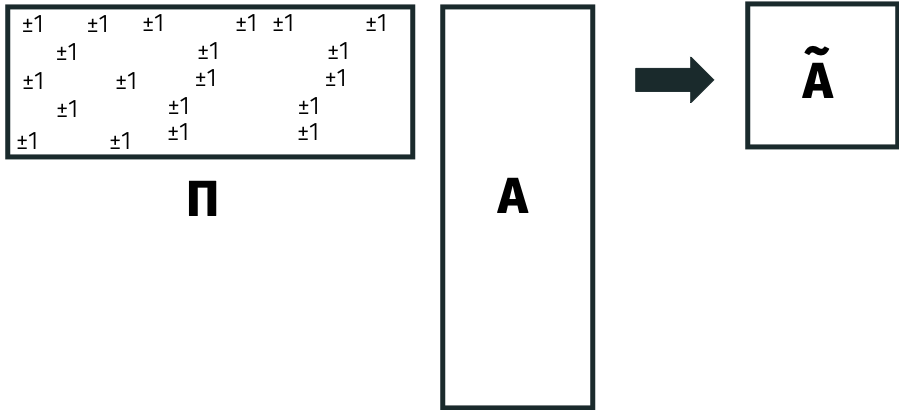
\includegraphics[width=.6\textwidth]{sparseJL.png}
		
		Typically using \emph{sparse} or \emph{structured} matrices instead of fully random JL matrices.
		
		Useful in many other applications two. For example, faster methods are often used in LSH systems to implement SimHash.
	\end{center}
\end{frame}

\begin{frame}[t]
	\frametitle{return to single vector problem}
	\textbf{Goal}: Develop methods that reduce a vector $\bv{x}\in \R^n$ down to $m \approx \frac{\log(1/\delta)}{\epsilon^2}$ dimensions in $o(mn)$ time and guarantee:
	\begin{align*}
		(1-\epsilon)\|\bv{x}\|_2^2 \leq \|\bs{\Pi}\bv{x}\|_2^2 \leq (1+\epsilon)\|\bv{x}\|_2^2
	\end{align*}
	\begin{center}
		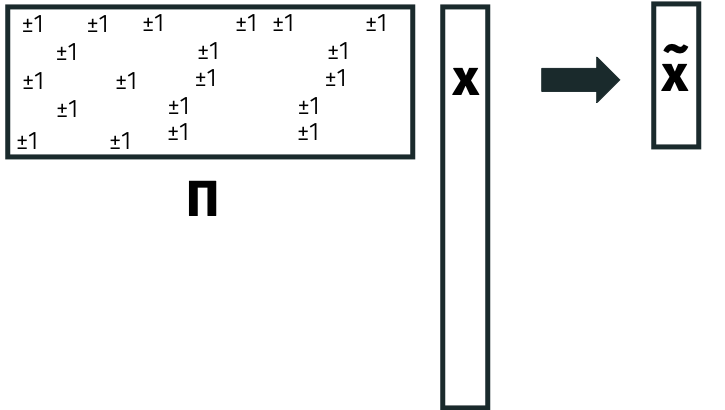
\includegraphics[width=.6\textwidth]{single_vec.png}
	\end{center}

Recall that once the bound above is proven, linearity lets us preserve things like $\|\bv{y} - \bv{z}\|_2^2$ or $\|\bv{Ax} - \bv{b}\|_2^2$ for all $\bv{x}$.
\end{frame}

\begin{frame}[t]
	\frametitle{the fast johnson-lindenstrauss transform}
	\small
	\begin{center}
		\textbf{Subsampled Randomized Hadamard Transform\footnote{One of my favorite randomized algorithms.} (SHRT) (Ailon-Chazelle, 2006)}
	\end{center}
	\begin{theorem}[The Fast JL Lemma]
		Let $\bs{\Pi} = \bv{SHD} \in \R^{m\times n}$ be a \emph{subsampled randomized Hadamard transform} with $m = O\left(\frac{\log(n/\delta)\log(1/\delta)}{\epsilon^2}\right)$ rows. Then for any fixed $\bv{x}$, 
		\begin{align*}
			(1-\epsilon)\|\bv{x}\|_2^2 \leq  \|\bs{\Pi}\bv{x}\|_2^2 \leq (1+\epsilon) \|\bv{x}\|_2^2
		\end{align*}
		with probability $(1-\delta)$ and $\bs{\Pi}\bv{x}$ can be computed in $O(n\log n)$ (nearly linear) time. 
	\end{theorem}
		Very little loss in embedding dimension compared to standard JL.
\end{frame}

\begin{frame}[t]
	\frametitle{solution for ``flat'' vectors}
	Let $\bv{S}$ be a \alert{random sampling matrix}. Every row contains a value of $s = \sqrt{n/m}$ in a single location, and is zero elsewhere. 
	
	\vspace{-1em}
		\begin{center}
		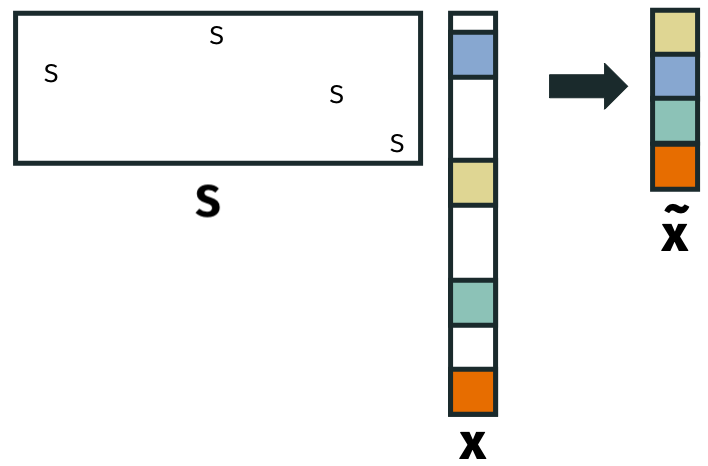
\includegraphics[width=.6\textwidth]{subsampling.png}
	\end{center}
If we take $m$ samples, $\tilde{\bv{x}}$ can be computed in $O(m)$ time. Woohoo!

\begin{center}
	\textbf{\alert{What is the problem with this approach?}}
\end{center}

%\begin{claim}
%		If $\bv{x}_i^2 \leq \frac{c}{n} \|\bv{x}\|_2^2$ for all $i$ then $m  = O(c\log(1/\delta)/\epsilon^2)$ samples suffices to ensure the $(1-\epsilon)\|\bv{x}\|_2^2 \leq \|\bv{S}\bv{x}\|_2^2 \leq (1+\epsilon)\|\bv{x}\|_2^2$ with probability $1-\delta$.
%\end{claim}
\end{frame}

\begin{frame}[t]
	\frametitle{vector sampling}
	Sampling only works well if $\bv{y} = \bv{A}\bv{x}$ is ``flat''. 
	\vspace{-.5em}
	\begin{center}
		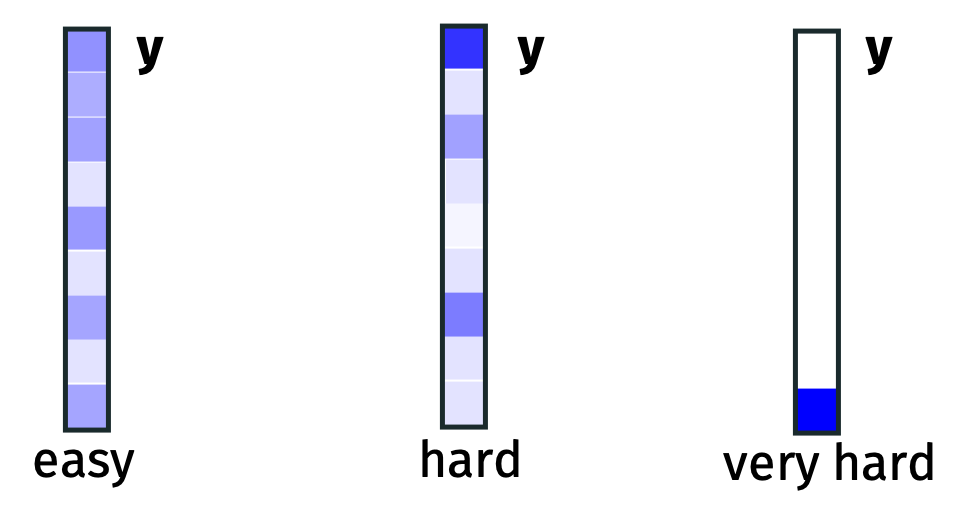
\includegraphics[width=.6\textwidth]{uniform_hard.png}
	\end{center}
	\vspace{-.5em}
	
\begin{claim}
		If $\bv{x}_i^2 \leq \frac{c}{n} \|\bv{x}\|_2^2$ for all $i$ then $m  = O(c\log(1/\delta)/\epsilon^2)$ samples suffices to ensure the $(1-\epsilon)\|\bv{x}\|_2^2 \leq \|\bv{S}\bv{x}\|_2^2 \leq (1+\epsilon)\|\bv{x}\|_2^2$ with probability $1-\delta$.
\end{claim}
This just follows from standard Hoeffding inequality. 
\end{frame}

%\begin{frame}[t]
%	\frametitle{variance analysis}	
%	Let $\tilde{\bv{y}}$ be the subsampled $\bv{y}$. Recall that, when sampling with probabilities $p_1, \ldots, p_n$, for $i = 1,\ldots, n$ we add $y_i$ to $\tilde{\bv{y}}$ with probability $p_i$ and reweight by $\frac{1}{\sqrt{p_i}}$. 
%	
%	\begin{align*}
%		\|\tilde{\bv{y}}\|_2^2 &= \sum_{i=1}^n \frac{y_i^2}{p_i}\cdot Z_i & &\text{where} & Z_i&= \begin{cases}
%			1 \text{ with probability $p_i$}\\
%			0 \text{ otherwise}\end{cases}
%	\end{align*}
%	
%	\begin{align*}
%		\Var[\|\tilde{\bv{y}}\|_2^2] =  \sum_{i=1}^n \frac{y_i^2}{p_i}\cdot \Var[Z_i] \leq  \sum_{i=1}^n \frac{y_i^4}{p_i^2}\cdot p_i = \frac{y_i^4}{p_i}
%	\end{align*}
%	
%	We set $p_i =  c\cdot \frac{y_i^2}{\|y\|_2^2}$ so get total variance:
%	\begin{align*}
%		\frac{1}{c}\|y\|_2^4
%	\end{align*}
%\end{frame}	
%
%\begin{frame}[t]
%	\frametitle{variance analysis}	
%	Using a Bernstein bound (or Chebyshev's inequality if you don't care about the $\delta$ dependence) we have that if $c = \frac{\log(1/\delta)}{\epsilon^2}$ then:
%	\begin{align*}
%		\Pr[\left|\|\tilde{\bv{y}}\|_2^2 - \|\bv{y}\|_2^2\right| \geq \epsilon \|\bv{y}\|_2^2] \leq \delta.
%	\end{align*}
%	
%	\vspace{4em}
%	The number of samples we take in expectation is:
%	\begin{align*}
%		\sum_{i=1}^n p_i = \sum_{i=1}^n c\cdot \frac{y_i^2}{\|y_i\|_2^2} = \frac{\log(1/\delta)}{\epsilon^2}. 
%	\end{align*}
%\end{frame}



\begin{frame}[t]
	\frametitle{the fast johnson-lindenstrauss transform}

\textbf{Key idea:} First multiply $\bv{x}$ by a ``mixing matrix'' $\bv{M}$ which ensures it cannot be too concentrated in one place. 

$\bv{M}$ will have the properties that 
\begin{enumerate}
	\item $\|\bv{M}\bv{x}\|_2^2 = \|\bv{x}\|_2^2$ \emph{exactly}.
	\item Every entry in $\bv{M}\bv{x}$ is bounded. I.e. $[\bv{M}\bv{x}]_i^2 \leq \frac{c}{n}\|\bv{M}\bv{x}\|_2^2$ for some factor $c$ to be determined.
	\item We will be able to multiply by $\bv{M}$ in $O(n \log n)$ time.
\end{enumerate}
 Then we will multiply by a subsampling matrix $\bv{S}$ to do the actual dimensionality reduction:
\begin{align*}
	\bs{\Pi}\bv{x} = \bv{SM}\bv{x}
\end{align*}
\end{frame}



\begin{frame}[t]
	\frametitle{the fast johnson-lindenstrauss transform}
	Good mixing matrices should look random:
	\begin{center}
	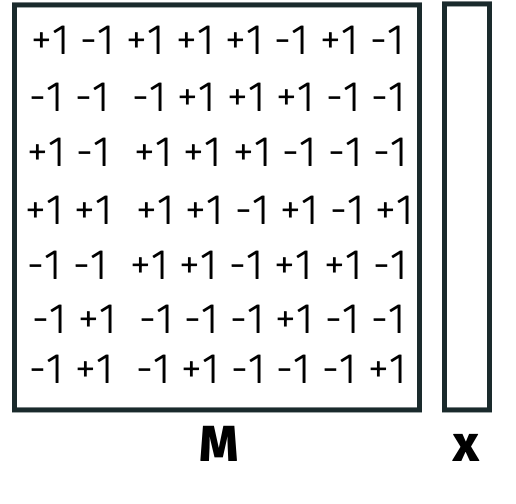
\includegraphics[width=.4\textwidth]{mixing.png}
	
	In fact, I claim to mix any $\bv{x}$ with high probability, $\bv{M}$ \emph{needs} to be chosen randomly. Why?
	
	\textbf{Hint:} Recall that $\|\bv{M}\bv{x}\|_2 = \|\bv{x}\|_2$, so $\bv{M}$ is orthogonal. 
	\end{center}
	
\end{frame}

\begin{frame}[t]
	\frametitle{the fast johnson-lindenstrauss transform}
	Good mixing matrices should look random:
	\begin{center}
		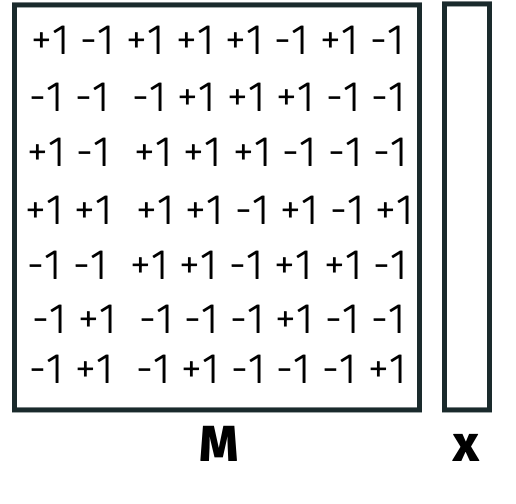
\includegraphics[width=.4\textwidth]{mixing.png}
		
		{But for this approach to work, we need to be able to compute $\bv{M}\bv{x}$ very quickly.} So we will use a \textbf{\alert{pseudorandom}} matrix instead.
	\end{center}
	
\end{frame}

\begin{frame}[t]
	\frametitle{the fast johnson-lindenstrauss transform}
	\begin{center}
		\textbf{Subsampled Randomized Hadamard Transform}
	\end{center}
	$\bs{\Pi} = \bv{SM}$ where $\bv{M} = \bv{H}\bv{D}$:
	\begin{itemize}
		\item $\bv{D} \in n \times n$ is a diagonal matrix with each entry uniform $\pm 1$.
		\item $\bv{H} \in n \times n$ is a \emph{Hadamard matrix}.
	\end{itemize}

The Hadarmard matrix is an \emph{orthogonal} matrix closely related to the discrete Fourier matrix. It has three critical properties: 
\begin{enumerate}
	\item $\|\bv{H}\bv{v}\|_2^2 = \|\bv{v}\|_2^2$ exactly. Thus $\|\bv{H}\bv{D}\bv{x}\|_2^2 = \|\bv{x}\|_2^2$ 
	\item $\|\bv{H}\bv{v}\|_2^2$ can be computed in $O(n\log n)$ time. 
	\item All of the entries in $\bv{H}$ have the same magnitude. I.e. the matrix is ``flat''/
\end{enumerate}
\end{frame}

\begin{frame}[t]
	\frametitle{hadamard matrices recursive definition}
	\textbf{Assume that $n$ is a power of $2$}. For $k = 0, 1, \ldots,$ the $k^\text{th}$ {Hadamard matrix} $\bv{H}_k$ is a $2^k \times 2^k$ matrix defined by:
	\begin{align*}
	H_0 &= 1 
	& H_1 &= \frac{1}{\sqrt{2}}\begin{bmatrix}1 & 1 \\ 1& -1 \end{bmatrix} 
	& H_2 &= \frac{1}{\sqrt{4}}\begin{bmatrix}1 & 1 & 1& 1 \\ 1 & -1 & 1& -1 \\ 1 & 1 & -1& -1 \\1 & -1 & -1& 1  \end{bmatrix} 
	\end{align*}
	\begin{align*}
	H_k &= \frac{1}{\sqrt{2}}\begin{bmatrix}H_{k-1} & H_{k-1}  \\ H_{k-1} & -H_{k-1}  \end{bmatrix}
	\end{align*}
	\begin{center}
		The $n\times n$ Hadamard matrix has all entries as $\pm \frac{1}{\sqrt{n}}$. 
	\end{center}
\end{frame}

\begin{frame}[t]
	\frametitle{hadamard matrices are orthogonal}
	\textbf{Property 1}: For any $k = 0, 1, \ldots$, we have $\|\bv{H}_k\bv{v}\|_2^2 = \|\bv{v}\|_2^2$ for all $\bv{v}$. I.e., $\bv{H}_k$ is orthogonal.
	
	
\end{frame}

\begin{frame}[t]
	\frametitle{hadamard matrices}
	\textbf{Property 2}: Can compute $\bs{\Pi}\bv{x} = \bv{SHD}\bv{x}$ in $O(n\log n)$ time. 
	\vspace{14em}

\end{frame}

\begin{frame}
	\frametitle{randomized hadamard transform}
	\textbf{Property 3}: The randomized Hadamard matrix is a good ``mixing matrix'' for smoothing out vectors. 
	
	\begin{figure}[h]
		\centering
		\begin{subfigure}[t]{0.3\textwidth}
			\centering
			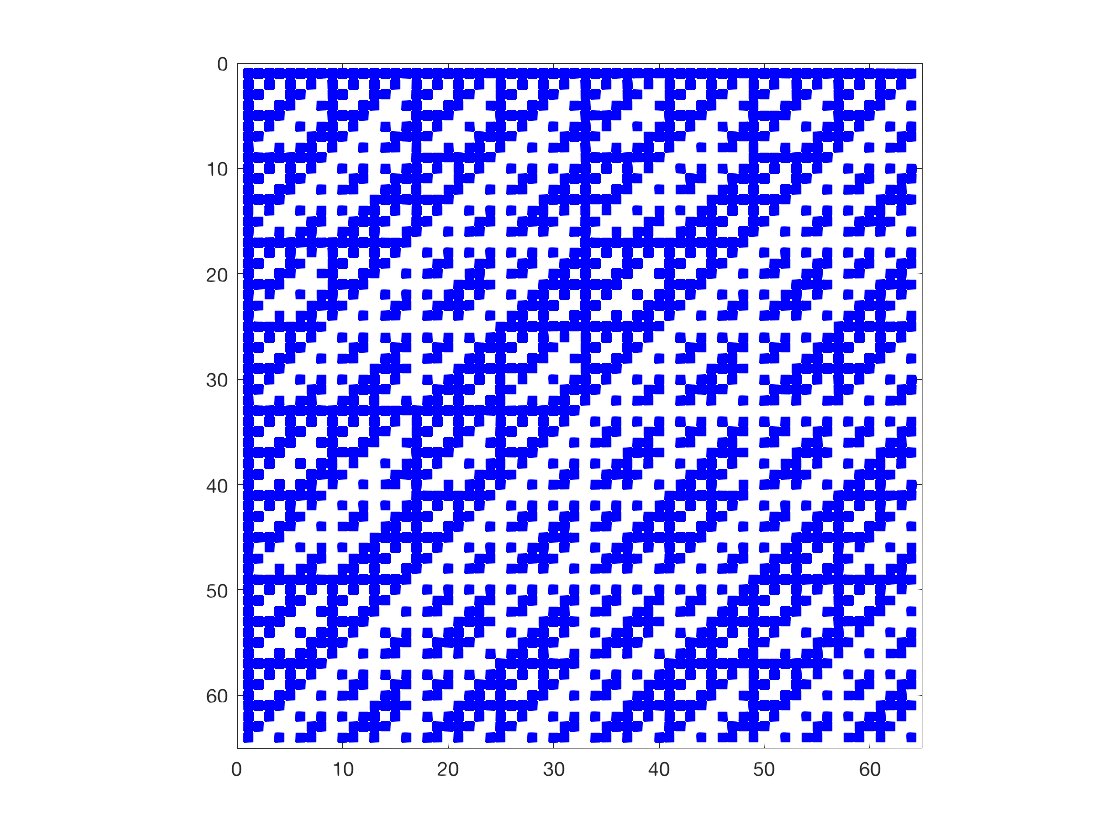
\includegraphics[width=\textwidth]{hadamard.png}
			\caption{Deterministic Hadamard matrix.}
		\end{subfigure}
		\begin{subfigure}[t]{0.3\textwidth}
			\centering
			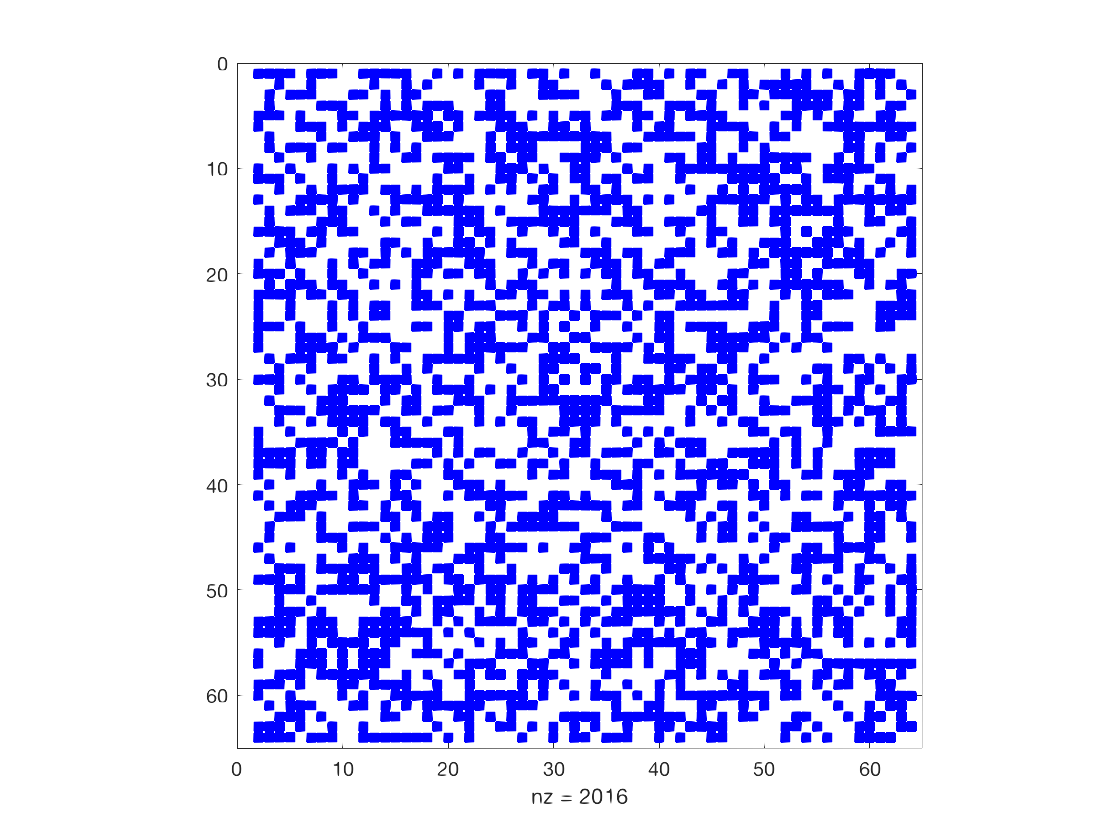
\includegraphics[width=\textwidth]{randomizedHadamard.png}
			\caption{Randomized Hadamard $\bv{PHD}$.}
		\end{subfigure}
		\begin{subfigure}[t]{0.3\textwidth}
			\centering
			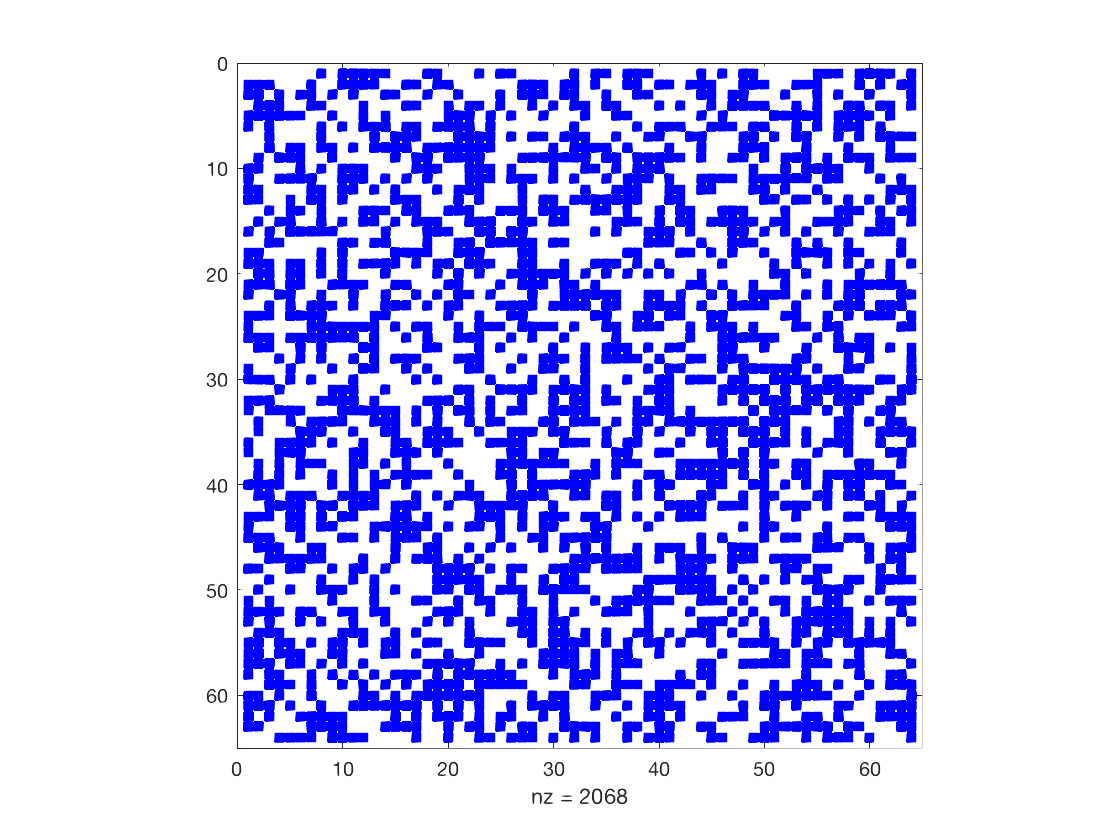
\includegraphics[width=\textwidth]{fullyRandom.png}
			\caption{Fully random sign matrix.}
		\end{subfigure}
	\caption{Blue squares are $1/\sqrt{n}$'s, white squares are $-1/\sqrt{n}$'s.}
	\end{figure}
Pseudorandom objects like this appear all the time in computer science! Error correcting codes, efficient hash functions, etc.
\end{frame}

\begin{frame}[t]
	\frametitle{randomized hadamard analysis}
	\begin{lemma}[SHRT mixing lemma]
		Let $\bv{H}$ be an $(n\times n)$ Hadamard matrix and $\bv{D}$ a random $\pm 1$ diagonal matrix. Let $\bv{z} = \bv{HD}\bv{x}$ for $\bv{x}\in \R^n$. With probability $1-\delta$, for all $i$ simultaneously,
		\begin{align*}
			z_i^2 \leq \frac{c\log(n/\delta)}{n} \|\bv{z}\|_2^2 
		\end{align*}
		for some fixed constant $c$. 
	\end{lemma}
	\alert{\textbf{The vector is very close to uniform with high probability}.} As we saw earlier, we can thus argue that $\|\bv{S}\bv{z}\|_2^2 \approx \|\bv{z}\|_2^2$. I.e. that:
	\begin{align*}
		\|\bs{\Pi}\bv{x}\|_2^2 = \|\bv{SHD}\bv{x}\|_2^2 \approx \|\bv{x}\|_2^2
	\end{align*}
\end{frame}

\begin{frame}[t]
	\frametitle{johnson-lindenstrauss with shrts}
	The main result then follows directly from our sampling result from earlier:
		\begin{theorem}[The Fast JL Lemma]
		Let $\bs{\Pi} = \bv{SHD} \in \R^{m\times n}$ be a subsampled randomized Hadamard transform with $m = O\left(\frac{\log(n/\delta)\log(1/\delta)}{\epsilon^2}\right)$ rows. Then for any fixed $\bv{x}$, 
		\begin{align*}
		(1-\epsilon)\|\bv{x}\|_2^2 \leq  \|\bs{\Pi}\bv{x}\|_2^2 \leq (1+\epsilon) \|\bv{x}\|_2^2
		\end{align*}
		with probability $(1-\delta)$. 
	\end{theorem}
\begin{center}
\end{center}
\end{frame}

\begin{frame}[t]
	\frametitle{randomized hadamard analysis}
	\textbf{SHRT mixing lemma proof:}
	Need to prove $(z_i)^2 \leq \frac{c\log(n/\delta)}{n} \|\bv{z}\|_2^2$. 
	
	Let $\bv{h}_i^T$ be the $i^\text{th}$ row of $\bv{H}$. ${z}_i = \bv{h}_i^T\bv{D}\bv{x}$ where:
	\begin{align*}
	\bv{h}_i^T\bv{D} = \frac{1}{\sqrt{n}}\begin{bmatrix} 1 & 1 & \ldots & -1 & -1 \end{bmatrix}
	\begin{bmatrix} 
		D_1 &  &  & \\ 
		& D_2  &  & \\ 
		& &  \ddots  & \\ 
		& &   &  D_n \\ 
		\end{bmatrix}
	\end{align*}
	where $D_1, \ldots, D_n$ are random $\pm 1$'s.
	
	This is equivalent to
	\begin{align*}
	\bv{h}_i^T\bv{D}  = \frac{1}{\sqrt{n}}\begin{bmatrix} R_1 & R_2 & \ldots & R_n \end{bmatrix}, 
	\end{align*}
where $R_1, \ldots, R_n$ are random $\pm 1$'s.

\end{frame}

\begin{frame}[t]
	\frametitle{randomized hadamard analysis}
	So we have, for all $i$,
	${z}_i = \bv{h}_i^T\bv{D}\bv{x} = \frac{1}{\sqrt{n}}\sum_{i=1}^n R_i x_i.$
	
	\begin{itemize}
	\item ${z}_i$ is a random variable with mean $0$ and variance $\frac{1}{n}\|\bv{x}\|_2^2$, which is a sum of independent random variables. 
	\end{itemize}
\end{frame}

\begin{frame}[t]
	\frametitle{randomized hadamard analysis}
	${z}_i$ is a random variable with mean $0$ and variance $\frac{1}{n}\|\bv{x}\|_2^2$, which is a sum of independent random variables. 
	\begin{itemize}
		\item By Central Limit Theorem, we expect that:
		\begin{align*}
			\Pr[|\bv{z}_i| \geq t\cdot \frac{\|\bv{x}\|_2}{\sqrt{n}}] \leq e^{-O(t^2)}. 
		\end{align*}
		\item Setting $t = \sqrt{\log(n/\delta)}$, we have for constant $c$, \begin{align*}\Pr\left[|\bv{z}_i| \geq c\sqrt{\frac{\log(n/\delta)}{n}}\|\bv{x}\|_2 \right] \leq \frac{\delta}{n}\end{align*}. 
		\item Applying a union bound to all $n$ entries of $\bv{z}$ gives the SHRT mixing lemma.
	\end{itemize}
\end{frame}


\begin{frame}[t]
	\frametitle{rademacher concentration}
	Can use Bernstein type concentration inequality to prove the bound:
	\begin{lemma}[Rademacher Concentration]
		Let ${R}_1, \ldots, R_n$ be Rademacher random variables (i.e. uniform $\pm 1$'s). Then for any vector $\bv{a}\in \R^n$,
		\begin{align*}
		\Pr\left[\sum_{i=1}^n R_i a_i \geq t \|\bv{a}\|_2 \right] \leq e^{-t^2/2}.
		\end{align*}
	\end{lemma}
This is called the \emph{Khintchine Inequality}. It is specialized to sums of scaled $\pm 1$'s, and is a bit tighter and easier to apply than using a generic Bernstein bound.
\end{frame}

\begin{frame} 
	\frametitle{finishing up}
	Recall that $\bv{z} = \bv{H}\bv{D}\bv{x}$.
	
	With probability $1-\delta$, we have that for all $i$,
	\begin{align*}
		z_i \leq \sqrt{\frac{c\log(n/\delta)}{n}}\|\bv{x}\|_2 = \sqrt{\frac{c\log(n/\delta)}{n}}\|\bv{z}\|_2.
	\end{align*} 
	
	As shown earlier, we can thus guarantee that:
	\begin{align*}
		(1-\epsilon)\|\bv{z}\|_2^2 \leq \|\bv{S}\bv{z}\|_2^2 \leq (1+\epsilon)\|\bv{z}\|_2^2
	\end{align*}
as long as $\bv{S}\in \R^{m\times n}$ is a random sampling matrix with
	\begin{align*}
	m = O\left(\frac{\log(n/\delta)\log(1/\delta)}{\epsilon^2}\right) \text{ rows}. 
	\end{align*}
	
	$\|\bv{S}\bv{z}\|_2^2 = \|\bv{SHD}\bv{x}\|_2^2 = \|\bs{\Pi}\bv{x}\|_2^2$ and $\|\bv{z}\|_2^2 = \|\bv{x}\|_2^2$, so we are done. 
\end{frame}

\begin{frame}[t]
	\frametitle{linear regression with SHRTs}

\textbf{Upshot for regression:} Compute $\bs{\Pi}\bv{A}$ in \alert{$O(nd\log n)$ time} instead of $O(nd^2)$ time. Compress problem down to $\tilde{\bv{A}}$ with $O(d^2)$ dimensions. 
\end{frame}

\begin{frame}[t]
	\frametitle{brief comment on other methods}
	$O(nd\log n)$ is nearly linear in the size of $\bv{A}$ when $\bv{A}$ is dense. 
	\vspace{1em}
	
	\textbf{Clarkson-Woodruff 2013, STOC Best Paper}: Let $O\left(\nnz(\bv{A})\right)$ be the number of non-zeros in $\bv{A}$. It is possible to compute $\tilde{\bv{A}}$ with $\poly(d)$ rows in:
	\begin{align*}
	O\left(\nnz(\bv{A})\right) \text{ time.}
	\end{align*}
	$\bs{\Pi}$ is chosen to be an ultra-sparse random matrix. Uses totally different techniques (you can't do JL + $\epsilon$-net). 
	
	Lead to a whole close of matrix algorithms (for regression, SVD, etc.) which run in time:
	\begin{align*}
		O\left(\nnz(\bv{A})\right)  + \poly(d,\epsilon).
	\end{align*}
\end{frame}

\begin{frame}[t]
	\frametitle{what were ailon and chazelle thinking?}
Simple, inspired algorithm that has been used for accelerating:
\begin{columns}
	\begin{column}{.5\textwidth}
		\footnotesize{
		\begin{itemize}
			\item Vector dimensionality reduction
			\item Linear algebra
			\item Locality sensitive hashing (SimHash)
			\item Randomized kernel learning methods.
		\end{itemize}
	}
	\end{column}
	\begin{column}{.5\textwidth}
		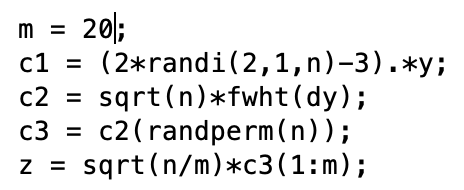
\includegraphics[width=\textwidth]{fastJL.png}
\end{column}
\end{columns}
\end{frame}

\begin{frame}[standout]
	\begin{center}
			\large break
		\end{center}
\end{frame}

\begin{frame}
		\frametitle{what were ailon and chazelle thinking?}
	The \emph{Hadamard Transform} is closely related to the \emph{Discrete Fourier Transform}.
	\begin{align*}
	\bv{F}_{j,k} &= e^{-2\pi i \frac{j\cdot k}{n}}, & \bv{F}^*\bv{F} &= \bv{I}.
	\end{align*}
	\begin{center}
		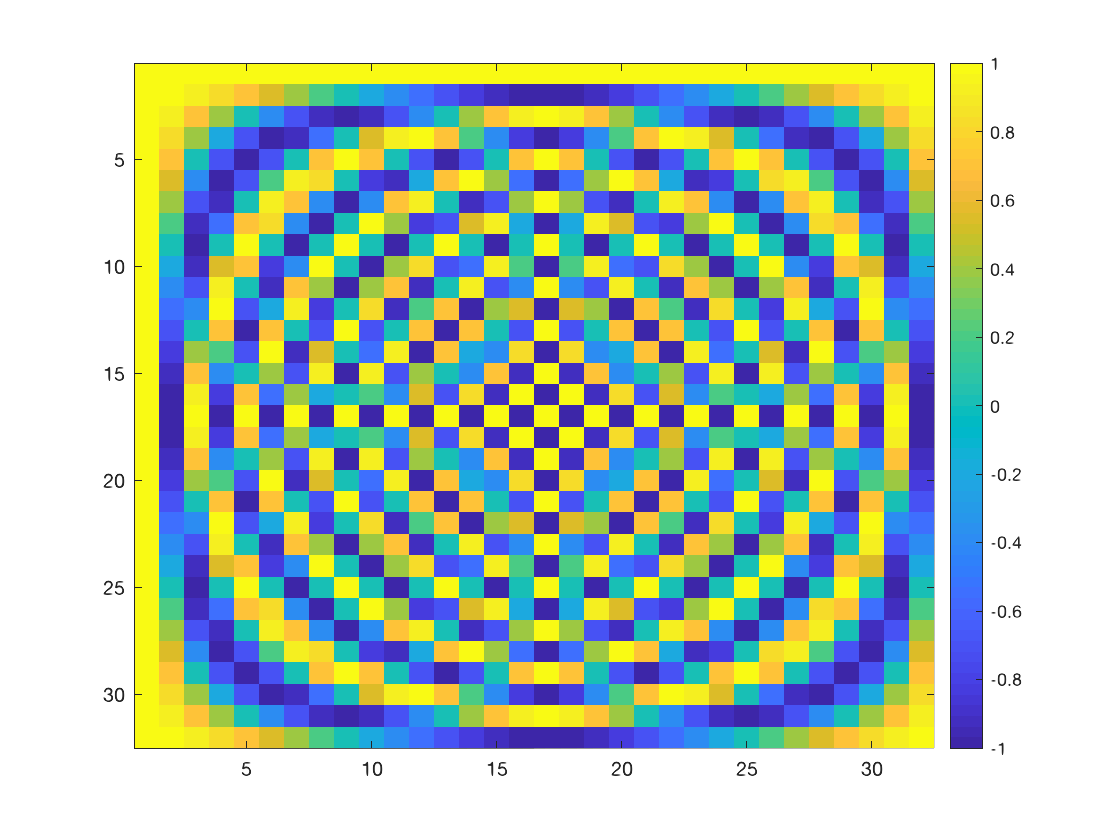
\includegraphics[width=.4\textwidth]{dft.png}
		\vspace{-1em}
		
		Real part of $\bv{F}_{j,k}$.
	\end{center}
	
	$\bv{F}\bv{y}$ computes the Discrete Fourier Transform of the vector $\bv{y}$. Can be computed in $O(n\log n)$ time using a divide and conquer algorithm (the Fast Fourier Transform).
\end{frame}

\begin{frame}
	\frametitle{fourier transform}
	The real part of $e^{-2\pi i \frac{j\cdot k}{n}}$ equals $cos(2\pi j \cdot k)$. So, the $j^\text{th}$ row of $\bv{F}$ looks like a cosine wave with frequency $2\pi j$. 

	Computing $\bv{F}\bv{x}$ computes inner products of $\bv{x}$ with a bunch of different frequencies, which can be used to decompose the vector into a sum of those frequencies.

	\vspace{-1em}
\begin{center}
	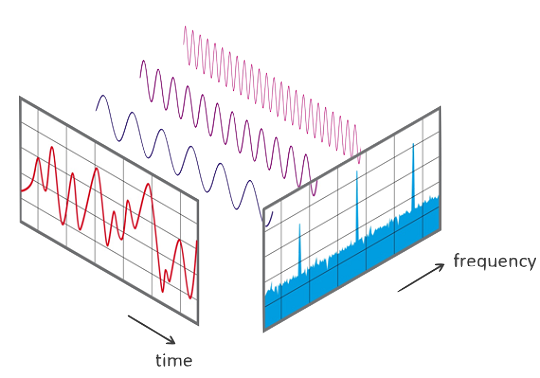
\includegraphics[width=.7\textwidth]{fourier_transform.png}
\end{center}
\end{frame}

\begin{frame}
	\frametitle{the uncertainty principal}
	\textbf{The Uncertainty Principal (informal):} A function and it's Fourier transform cannot both be concentrated. 
	\vspace{1em}
	\begin{columns}
		\begin{column}{.5\textwidth}
			\centering
			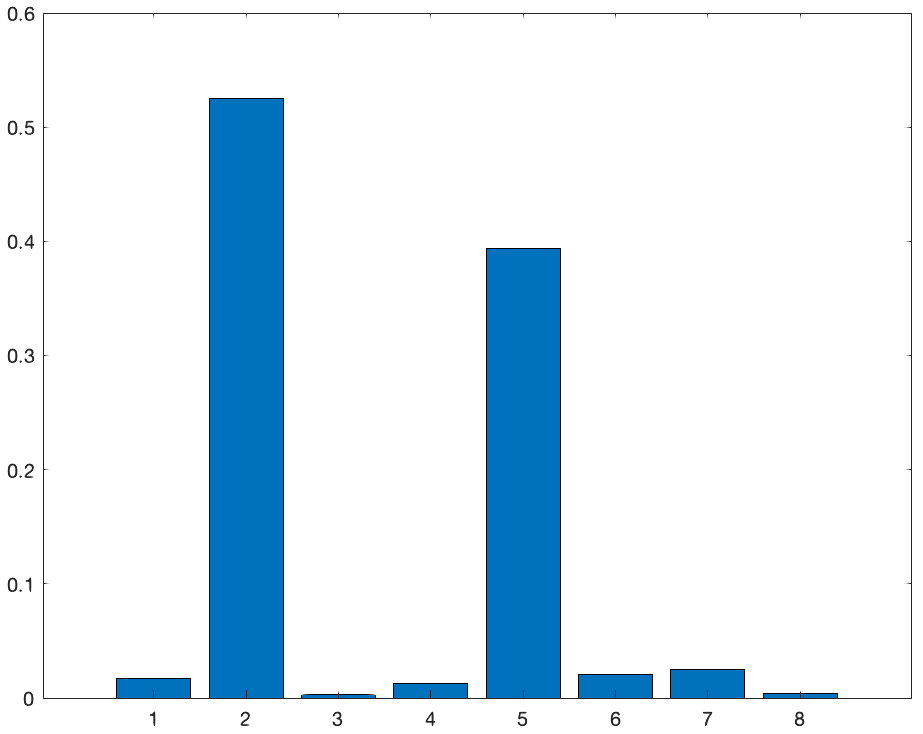
\includegraphics[width=.8\textwidth]{y.png}
			
			Vector $\bv{y}.$
		\end{column}
			\begin{column}{.5\textwidth}
		\centering
		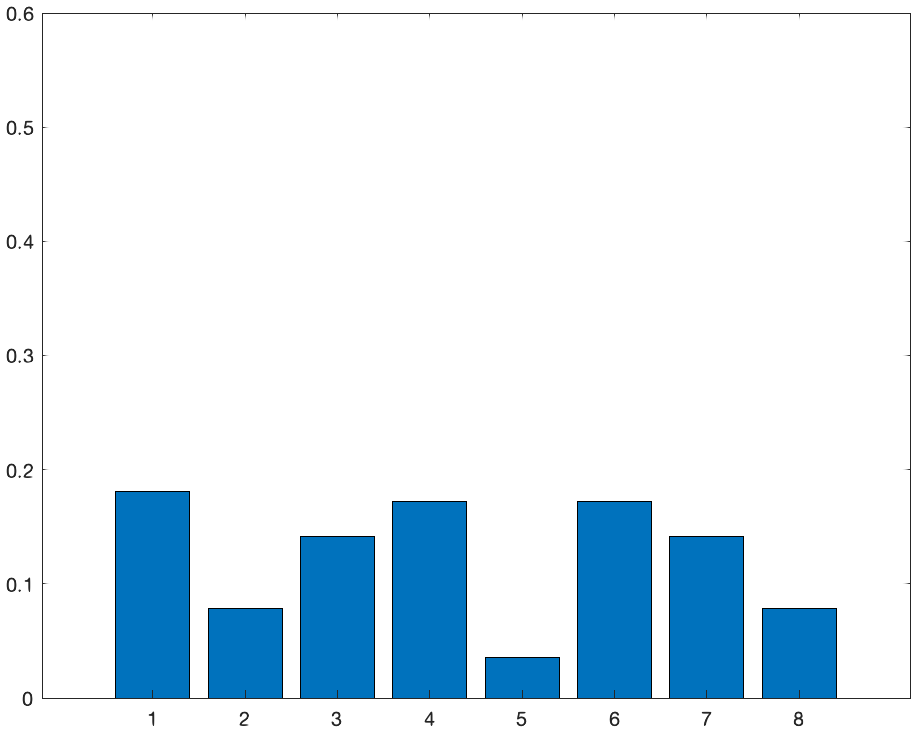
\includegraphics[width=.8\textwidth]{Fy.png}
		
		Fourier transform $\bv{Fy}.$
	\end{column}
	\end{columns}
%\textbf{We will talk about this a lot more next class. It is also the main idea behind \alert{compressed sensing} and \alert{sparse recovery}.}
\end{frame}


\begin{frame}
	\frametitle{the uncertainty principal}
	Sampling does not preserve norms, i.e. $\|\bv{S}\bv{y}\|_2 \not\approx \|\bv{y}\|_2$ when $\bv{y}$ has a few large entries. 
	
	Taking a Fourier transform exactly eliminates this hard case, without changing $\bv{y}$'s norm.
	
	\begin{center}
		One of the central tools in the field of \alert{\textbf{sparse recovery}} aka \alert{\textbf{compressed sensing.}}
	\end{center}
\end{frame}

\begin{frame}
	\frametitle{sparse recovery/compressed sensing problem setup}
	\textbf{Goal:} Recover a vector $\bv{x}$ from linear measurements.

	Choose $\bv{A}\in\R^{m \times n}$ with $m < n$. Assume we can access $\bv{b} = \bv{A}\bv{x}$ via some black-box measurement process. Try to recover $\bv{x}$ from the information in $\bv{b}$. 
	\begin{center}
		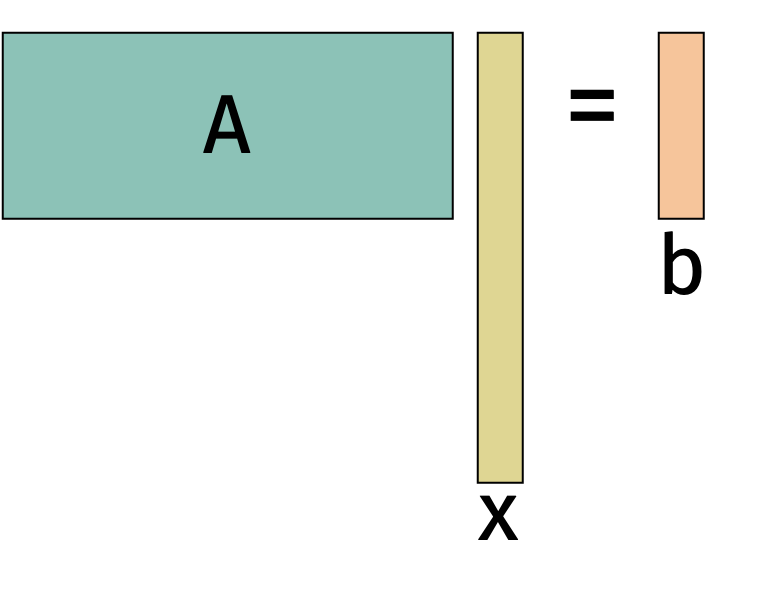
\includegraphics[width=.4\textwidth]{underdetermined.png}
	\end{center}
	\vspace{-1em}
	\begin{itemize}
		\item Infinite possible solutions $\bv{y}$ to $\bv{A}\bv{y} = \bv{b}$, so in general, it is impossible to recover $\bv{x}$ from $\bv{b}$. 
		\item Can often be possible if $\bv{x}$ has additional structure!
	\end{itemize}
\end{frame}

\begin{frame}
	\frametitle{example application: single pixel camera}
	\textbf{Typical acquisition of image by camera:}
	\begin{center}
		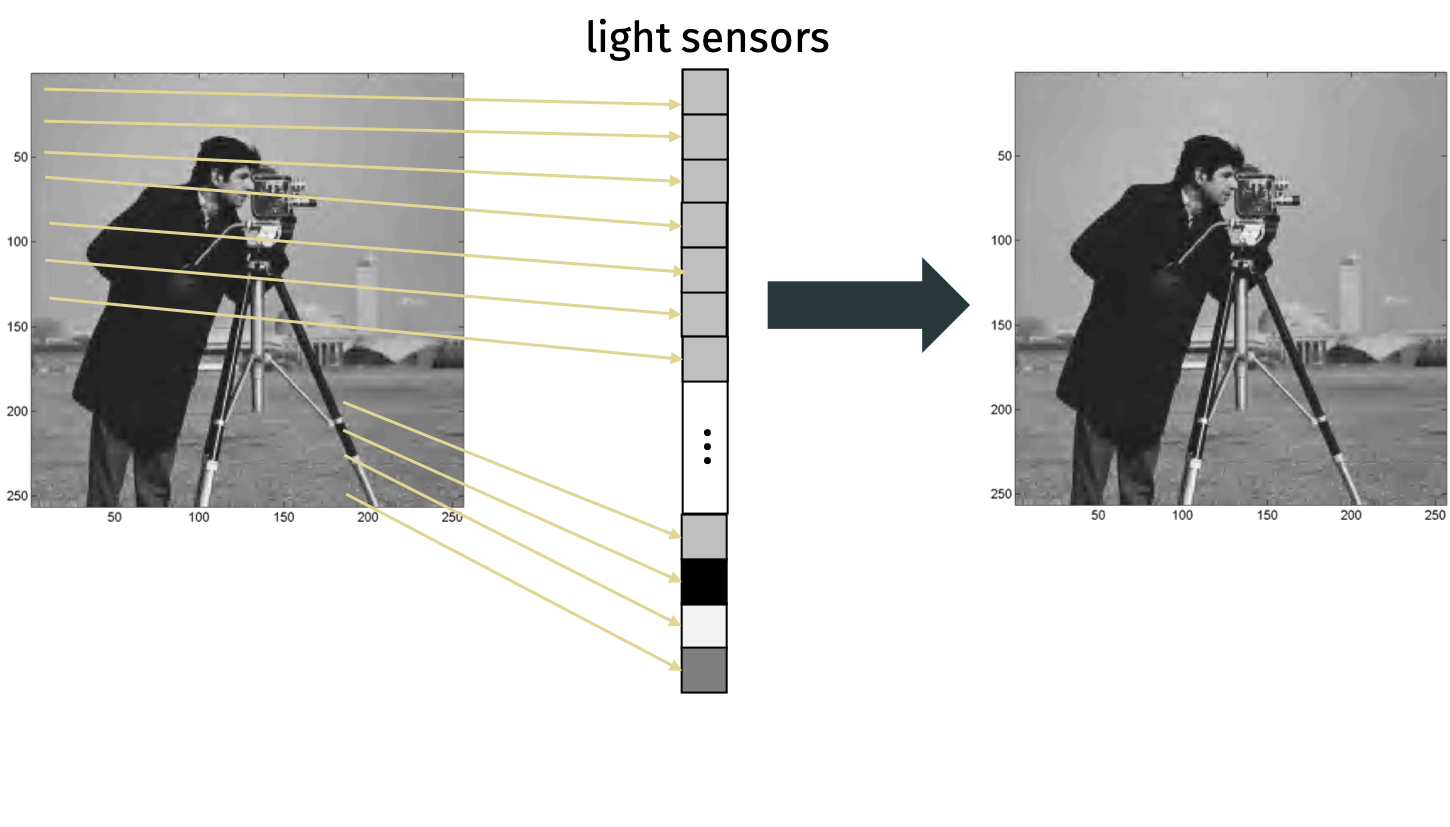
\includegraphics[width=.8\textwidth]{typicalCamera.png}
		
		Requires one image sensor per pixel captured.
	\end{center}
\end{frame}

\begin{frame}
	\frametitle{example application: single pixel camera}
	\textbf{Compressed acquisition of image:}
	\begin{center}
		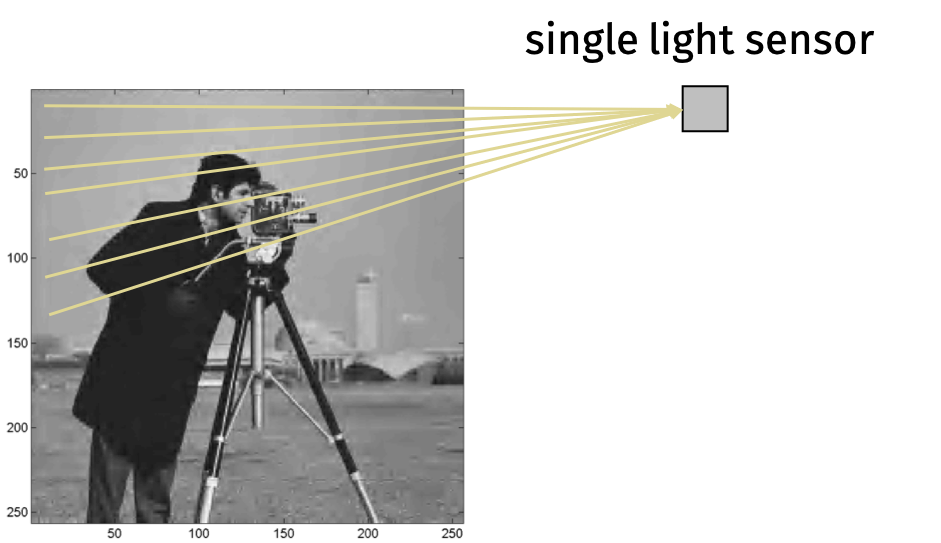
\includegraphics[width=.6\textwidth]{singlePixelCamera.png}
		\begin{align*}
			b = \sum_{i=1}x_i  = \begin{bmatrix}\frac{1}{n} &\frac{1}{n} &\ldots& \frac{1}{n}\end{bmatrix}\begin{bmatrix}x_1 \\x_2 \\\vdots\\ x_n\end{bmatrix}
		\end{align*}
		Does not provide very much information about the image. 
	\end{center}
\end{frame}

\begin{frame}
	\frametitle{example application: single pixel camera}
	\begin{center}
		\textbf{But you can get more information from other linear measurements via masking!}
		
		\vspace{-.5em}
		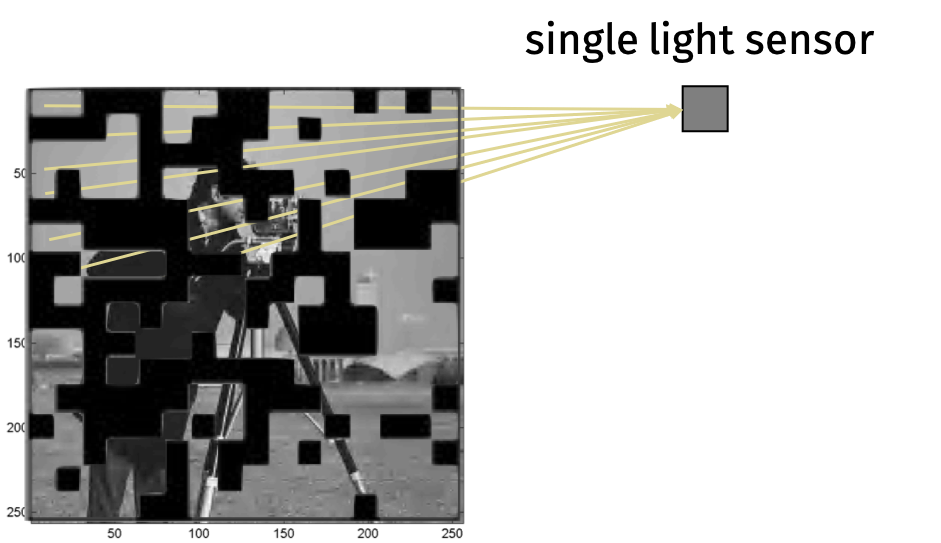
\includegraphics[width=.6\textwidth]{maskedImage.png}
		\vspace{-1.5em}
		\begin{align*}
			b_i =\langle \bv{a}_i,\bv{x} \rangle = \begin{bmatrix}0 &1 & 0 & 0 \ldots& 1\end{bmatrix}\begin{bmatrix}x_1 \\x_2 \\\vdots\\ x_n\end{bmatrix}
		\end{align*}
	\end{center}
	Piece together many of these masked measurements, and can recover the whole image!
\end{frame}

\begin{frame}
	\frametitle{example application: single pixel camera}
	\textbf{Applications in:}
	\begin{itemize}
		\item Imaging outside of the visible spectrum (more expensive sensors).
		\item Microscopy.
		\item Other scientific imaging.
		\item We will discuss other applications shortly.
	\end{itemize}
	\begin{center}
		\alert{\textbf{The theory we will discuss does not exactly describe these problems, but has been very valuable in modeling them.}}
	\end{center}
\end{frame}

\begin{frame}
	\frametitle{sparsity recovery/compressed sensing}
	\textbf{Need to make some assumption to solve the problem.}
	Given $\bv{A}\in\R^{m \times n}$ with $m < n$, $\bv{b} \in \R^m$, want to recover  $\bv{x}$.
	\begin{itemize}
		\item \alert{Assume $\bv{x}$ is $k$-sparse for small $k$. $\|\bv{x}\|_0 = k$.}
	\end{itemize}
	\vspace{-1em}
	\begin{center}
		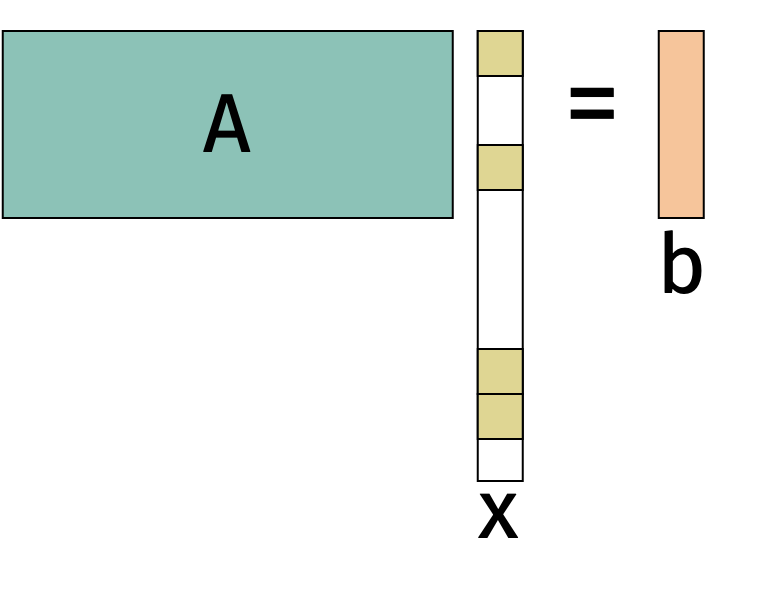
\includegraphics[width=.5\textwidth]{sparseRegressioon.png}
	\end{center}
	\vspace{-2em}
	\begin{itemize}
		\item In many cases can recover $\bv{x}$ with $\ll n$ rows. In fact, often $\sim O(k)$ suffice.
	\end{itemize}
\end{frame}

\begin{frame}
 \frametitle{sparsity assumption}
	\begin{center}
		\textbf{Is sparsify a reasonable assumption?}

		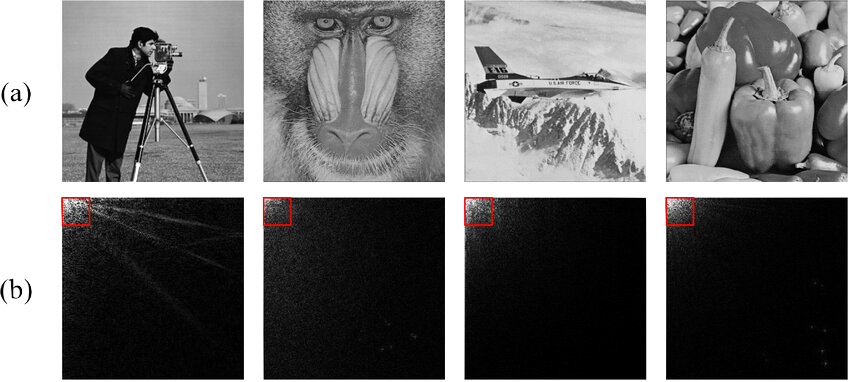
\includegraphics[width=.7\textwidth]{dct_basis.png}
		\end{center}
		For some of the approachs we will discuss, it suffices to assume that $\bv{x}$ is sparse in any fixed (and known) basis. I.e. that $\bv{V}\bv{x}$ is sparse for some $n\times n$ orthogonal $\bv{V}$. E.g. images are sparse in the Discrete Cosine Transform basis.

		Sparsity is a starting point for considering other more complex structure.
\end{frame}


\begin{frame}
	\frametitle{requirements for measurement matrix}
	What matrices $\bv{A}$ would definitely not allow us to recover $\bv{x}$?
	\begin{center}
		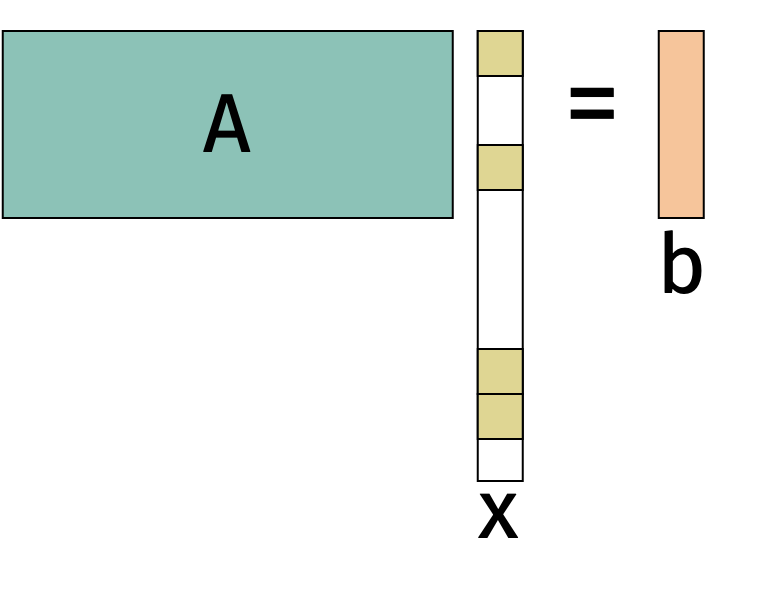
\includegraphics[width=.5\textwidth]{sparseRegressioon.png}
	\end{center}
\end{frame}

\begin{frame}
	\frametitle{assumptions on measurement matrix}
	\textbf{Many ways to formalize our intuition}
	\begin{itemize}
		\item $\bv{A}$ has \alert{\emph{Kruskal rank}} $r$. All sets of $r$ columns in $\bv{A}$ are linearly independent.
		\begin{itemize}
			\item Recover vectors $\bv{x}$ with sparsity $k = r/2$. 
		\end{itemize}
		\item $\bv{A}$ is \alert{\emph{$\mu$-incoherent}}. $|\bv{A}_i^T\bv{A}_j| \leq \mu \|\bv{A}_i\|_2 \|\bv{A}_j\|_2$ for all columns $\bv{A}_i, \bv{A}_j$, $i\neq j$. 
		\begin{itemize}
			\item Recover vectors $\bv{x}$ with sparsity $k = 1/\mu$. 
		\end{itemize}
		\item \textbf{Focus today}: $\bv{A}$ obeys the \alert{\emph{Restricted Isometry Property}}.
	\end{itemize}
\end{frame}

\begin{frame}
	\frametitle{restricted isometry property}
	\begin{definition}[$(q,\epsilon)$-Restricted Isometry Property]
		A matrix $\bv{A}$ satisfies $(q,\epsilon)$-RIP if, for all $\bv{x}$ with $\|\bv{x}\|_0 \leq q$, 
		\begin{align*}
			(1-\epsilon)\|\bv{x}\|_2^2 \leq \|\bv{A}\bv{x}\|_2^2 \leq  (1+\epsilon)\|\bv{x}\|_2^2.
		\end{align*}
	\end{definition}
	\begin{itemize}
		\item Johnson-Lindenstrauss type condition.
		\item $\bv{A}$ preserves the norm of all $q$ sparse vectors, instead of the norms of a fixed discrete set of vectors, or all vectors in a subspace (as in subspace embeddings).
		\item \textbf{Preview:} A random matrix $\bv{A}$ with $\sim O(q\log(n/q))$ rows satisfies RIP.
	\end{itemize}
\end{frame}

\begin{frame}[t]
	\frametitle{first sparse recovery result}
	\begin{theorem}[$\ell_0$-minimization]
		Suppose we are given $\bv{A} \in \R^{m\times n}$ and $\bv{b} = \bv{A}\bv{x}$ for an unknown $k$-sparse $\bv{x} \in \R^n$.
		If $\bv{A}$ is $(2k,\epsilon)$-RIP for any $\epsilon < 1$ then $\bv{x}$ is the \emph{unique} minimizer of:
		\begin{align*}
			\min &\|\bv{z}\|_0 & &\text{subject to} & \bv{A}\bv{z} &= \bv{b} .
		\end{align*}
	\end{theorem}
	\begin{itemize}
		\item Establishes that \emph{information theoretically} we can recover $\bv{x}$. Solving the $\ell_0$-minimization problem is computationally difficult, requiring $O(n^k)$ time. We will address faster recovery shortly.
	\end{itemize}
\end{frame}

\begin{frame}[t]
	\frametitle{first sparse recovery result}
	\textbf{Claim:} If $\bv{A}$ is $(2k,\epsilon)$-RIP for any $\epsilon < 1$ then $\bv{x}$ is the \emph{unique} minimizer of $\min_{\bv{A}\bv{z} = \bv{b}}\|\bv{z}\|_0$.
	
	\textbf{Proof:} By contradiction, assume there is some $\bv{y} \neq \bv{x}$ such that $\bv{Ay=b}$, $\|\bv{y}\|_0 \leq \|\bv{x}\|_0$. 
	
\end{frame}

\begin{frame}[t]
	\frametitle{robustness}
	\textbf{Important note:} \alert{There are {robust versions}} of this theorem and the others we will discuss. These are much more important practically. Here's a flavor of a robust result:
	\begin{itemize}
		\item Suppose $\bv{b} = \bv{A}(\bv{x} + \bv{e})$ where $\bv{x}$ is $k$-sparse and $\bv{e}$ is dense but has bounded norm.
		\item Recover some $k$-sparse $\tilde{\bv{x}}$ such that:
		\begin{align*}
			\|\tilde{\bv{x}} - \bv{x}\|_2 \leq\|\bv{e}\|_1
		\end{align*} 
		or even 
		\begin{align*}
			\|\tilde{\bv{x}} - \bv{x}\|_2 \leq O\left(\frac{1}{\sqrt{k}}\right) \|\bv{e}\|_1.
		\end{align*} 
	\end{itemize}
\end{frame}

\begin{frame}[t]
	\frametitle{robustness}
	We will not discuss robustness in detail, but along with computational considerations, it is a big part of what has made compressed sensing such an active research area in the last 20 years. Non-robust compressed sensing results have been known for a long time:
	
	\begin{center}
		\emph{Gaspard Riche de Prony}, \textit{Essay experimental et analytique: sur les lois de la dilatabilite
			de fluides elastique et sur celles de la force expansive de la vapeur de l’alcool, a differentes
			temperatures.} Journal de l’Ecole Polytechnique, 24–76. \textbf{1795}.
	\end{center}
	
\end{frame}

\begin{frame}
	\frametitle{restricted isometry property}
	\begin{center}
		\textbf{What matrices satisfy this property?}
	\end{center}
	\begin{itemize}
		\item Random Johnson-Lindenstrauss matrices (Gaussian, sign, etc.) with $m = O(\frac{k\log(n/k)}{\epsilon^2})$ rows are $(k,\epsilon)$-RIP. 
		%		\item Uniformly subsampled Fourier matrices with $O(q \log^3 n / \epsilon^2)$ rows \cite{rv08} (or see \cite{regev}). You have seen some of the tools to prove this. In  Lecture 11 we proved that a subsampled Hadamard matrix, which is a type of Fourier matrix, can be used to give the $JL$ gaurantee. Your Homework 3 argument would thus apply to these matrices as well. Proving RIP for actual Fourier matrices isn't too much of a leap.
		%		\item Explicit deterministic constructions with $O(q^2)$ rows (and slightly better \cite{ripdetermin}). Whether or not $O(q\log n)$ is possible with a deterministic construction is a major open question.
	\end{itemize}
	
	Some real world data may look random, but this is also a useful observation algorithmically when we want to \emph{design} $\bv{A}$.
\end{frame}



\begin{frame}
	\frametitle{the discrete fourier matrix}
	The $n \times n$ discrete Fourier matrix $\bv{F}$ is defined:
	\begin{align*}
		F_{j,k} = e^{\frac{-2\pi i}{n}j\cdot k}, 
	\end{align*}
	where $i = \sqrt{-1}$. Recall  $e^{\frac{-2\pi i}{n}j\cdot k} = cos(2\pi j k/n) - i \sin(2\pi j k/n)$.
	\begin{center}
		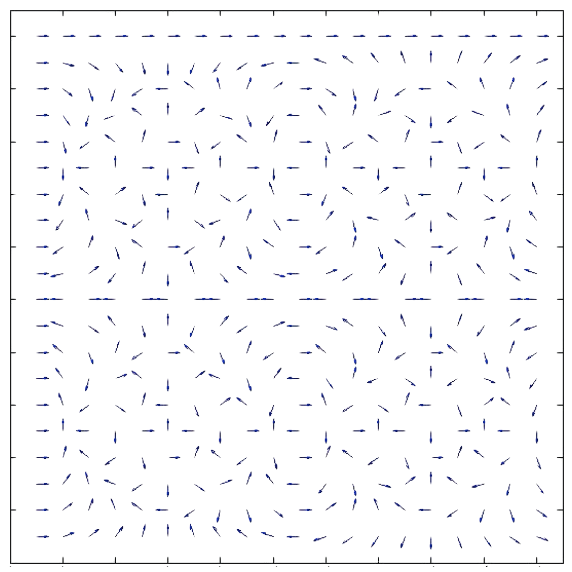
\includegraphics[width=.4\textwidth]{dftMatrix.png}
	\end{center}
\end{frame}

\begin{frame}
	\frametitle{pseudorandom rip matrices}
	In many applications can compute measurements of the form $\bv{Ax} = \bv{S}\bv{F}\bv{x}$, where $\bv{F}$ is the Discrete Fourier Transform matrix (what an FFT computes) and $\bv{S}$ is a subsampling matrix. 
	\begin{center}
		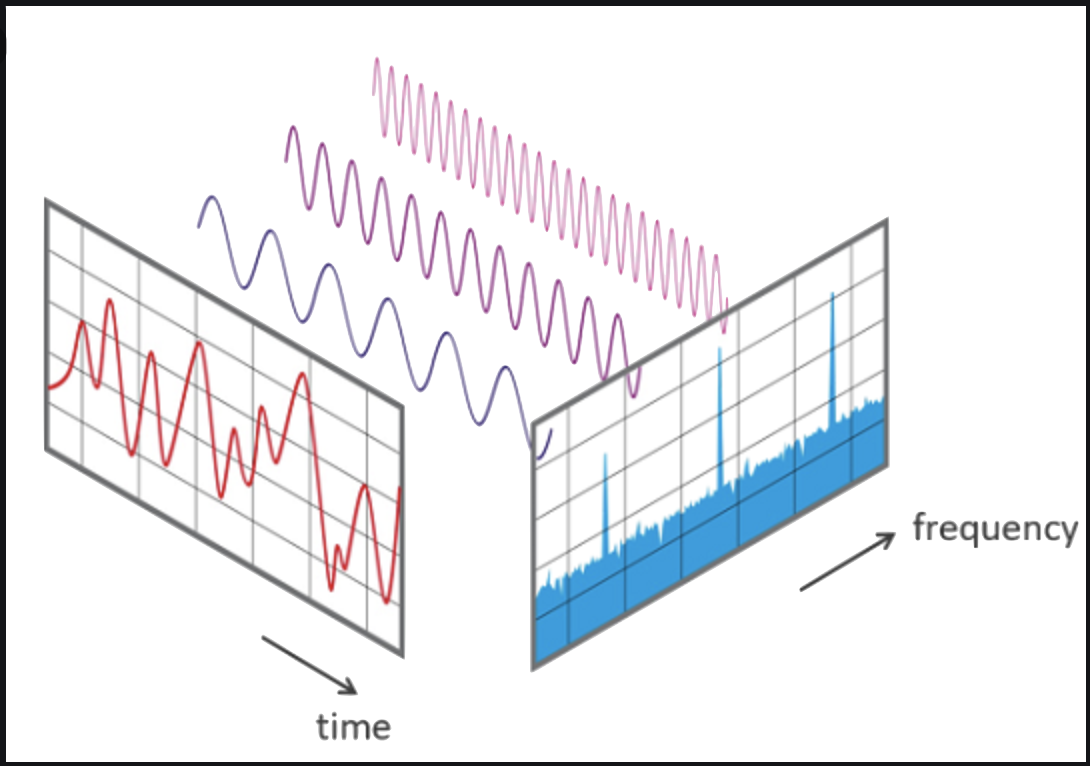
\includegraphics[width=.4\textwidth]{dftExample.png}
		
		$\bv{F}$ decomposes $\bv{x}$ into different frequencies: $[\bv{F}\bv{x}]_j$ is the component with frequency $j/n$. 
		
%		Because $\bv{F}^*\bv{F} = \bv{I}$, $\bv{F}^*\bv{F}\bv{x}= \bv{x}$, so we can recover $\bv{x}$ if we have access to its DFT. $\bv{F}\bv{x}$.  
	\end{center}
	
\end{frame}

\begin{frame}
	\frametitle{the discrete fourier matrix}
	If $\bv{A} = \bv{SF}$ is a subset of rows from $\bv{F}$, then $\bv{A}\bv{x}$ is a subset of random frequency components from $\bv{x}$'s discrete Fourier transform. 
	
	In many scientific applications, we can collect entries of $\bv{F}\bv{x}$ one at a time for some unobserved data vector $\bv{x}$. 
\end{frame}

\begin{frame}
	\frametitle{application: medical imaging}
	\begin{center}
		\alert{Warning: very cartoonish explanation of very complex problem.}		
	\end{center}
		\vspace{-1em}
	\textbf{Medical Imaging (MRI)}
	\begin{center}
		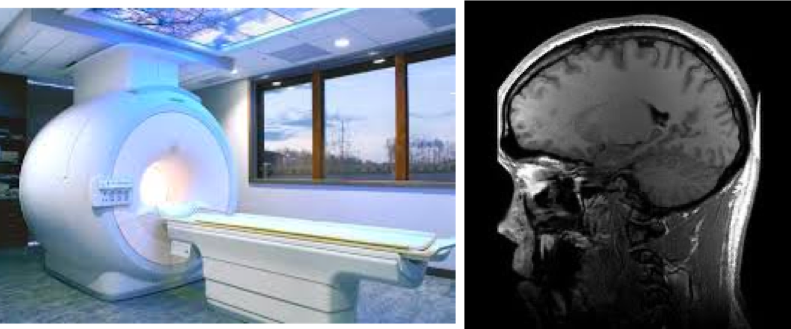
\includegraphics[width=.6\textwidth]{medicalImages.png}
	\end{center}
	
	\begin{center}
		How do we measure entries of Fourier transform $\bv{Fx}$? 		Blast the body with sounds waves of varying frequency.
	\end{center}

	\begin{itemize}
	\item Especially important when trying to capture something moving (e.g. lungs, baby, child who can't sit still). 
	\item Can also cut down on high power requirements.
\end{itemize}
\end{frame}


\begin{frame}
	\frametitle{application: geophysics}
	\begin{center}
		\alert{Warning: very cartoonish explanation of very complex problem.}
	\end{center}
	\textbf{Understanding what material is beneath the crust:}
	\begin{center}
		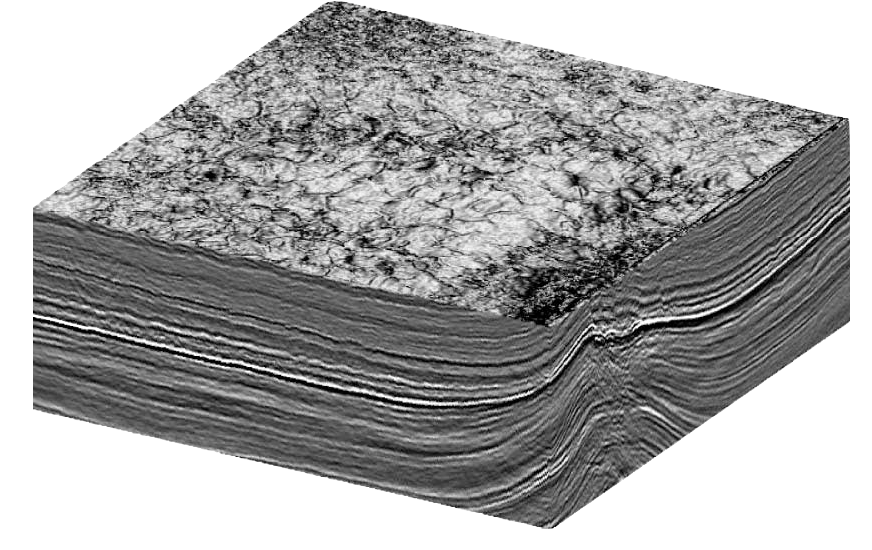
\includegraphics[width=.4\textwidth]{cube.png}
	\end{center}
\end{frame}

\begin{frame}
	\frametitle{application: geophysics}
	\begin{center}
		\textbf{Vibrate the earth at different frequencies!} And measure the response.
		
		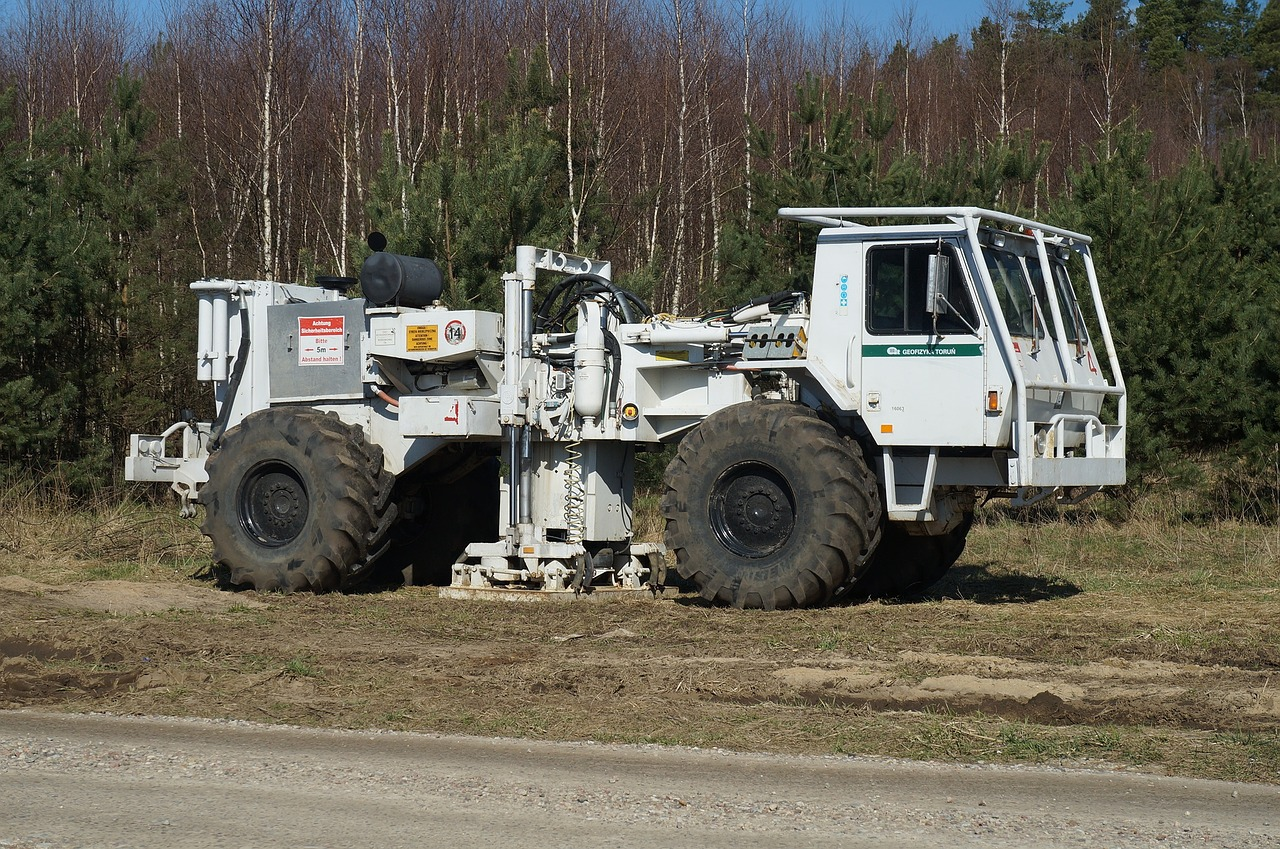
\includegraphics[width=.4\textwidth]{vibroseis.jpg}
		
		Vibroseis Truck
	\end{center}
	
	Can also use airguns, controlled explorations, vibrations from drilling, etc. The fewer measurements we need from $\bv{F}\bv{x}$, the cheaper and faster our data acquisition process becomes. 
\end{frame}



\begin{frame}
	\frametitle{restricted isometry property}
	Setting $\bv{A}$ to contain a random $m \sim O\left(\frac{k \log^2 k \log n}{\epsilon^2}\right)$ rows of the discrete Fourier matrix $\bv{F}$ yields a matrix that with high probability satisfies $(k,\epsilon)$-RIP. [Haviv, Regev, 2016]. 
	
	Improves on a long line of work: Cand\`{e}s, Tao, Rudelson, Vershynin, Cheraghchi, Guruswami, Velingker, Bourgain.
	
	\begin{center}
		Proving this requires similar tools to analyzing subsampled Hadamard transforms!
	\end{center}
\end{frame}

\begin{frame}
	\frametitle{restricted isometry property}
	\begin{definition}[$(q,\epsilon)$-Restricted Isometry Property -- Candes, Tao '05]
		A matrix $\bv{A}$ satisfies $(q,\epsilon)$-RIP if, for all $\bv{x}$ with $\|\bv{x}\|_0 \leq q$, 
		\begin{align*}
			(1-\epsilon)\|\bv{x}\|_2^2 \leq \|\bv{A}\bv{x}\|_2^2 \leq  (1+\epsilon)\|\bv{x}\|_2^2.
		\end{align*}
	\end{definition}
	The vectors that can be written as $\bv{A}\bv{x}$ for $q$ sparse $\bv{x}$ lie in a \emph{union of $q$ dimensional linear subspaces}:
	\begin{center}
		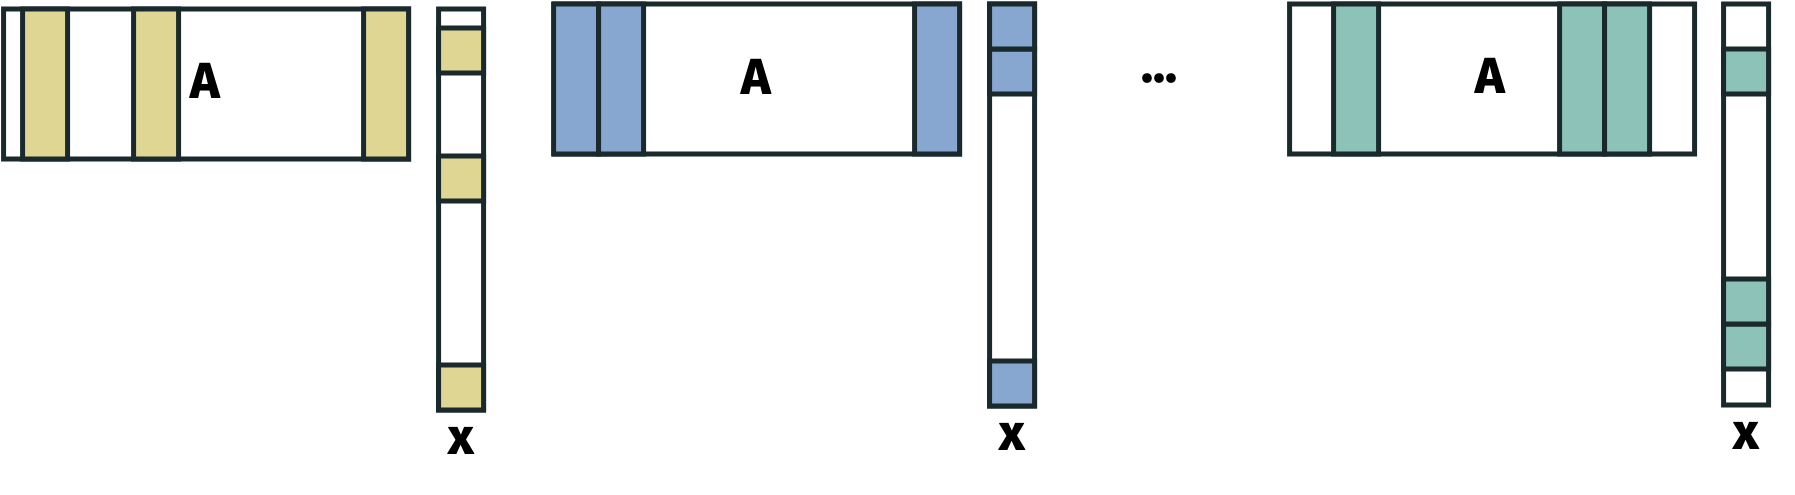
\includegraphics[width=\textwidth]{subspaces1.png}
	\end{center}
\end{frame}

\begin{frame}[t]
	\frametitle{restricted isometry property}
	\begin{center}
		\textbf{Candes, Tao 2005}: A random JL matrix with $O(q\log (n/q)/\epsilon^2)$ rows satisfies $(q,\epsilon)$-RIP with high probability.
		
		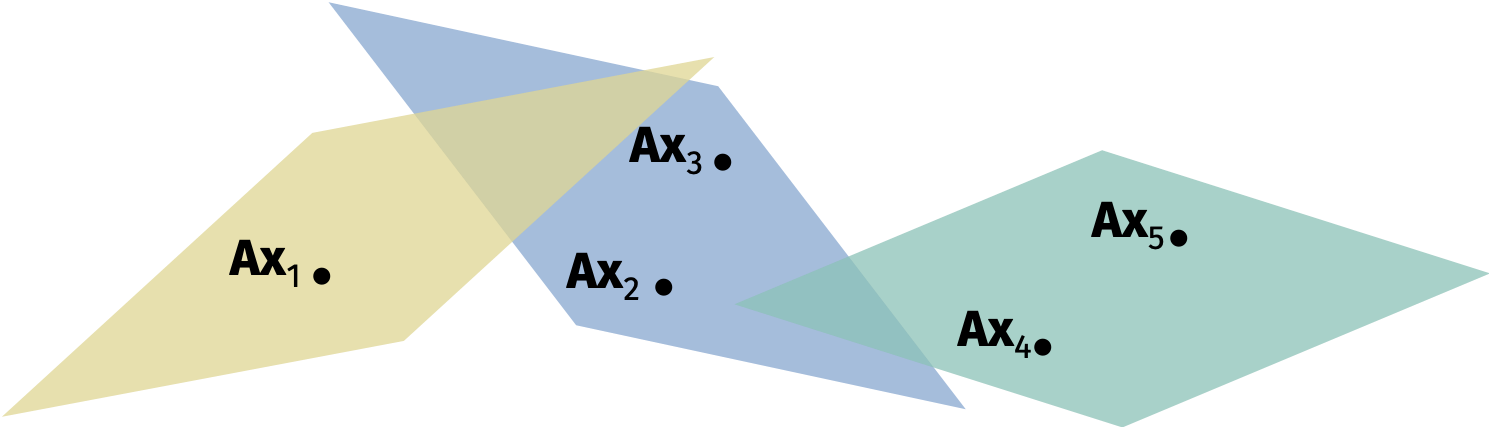
\includegraphics[width=\textwidth]{subspaces.png}
		
		Any ideas for how you might prove this? I.e. prove that a random matrix preserves the norm of every $\bv{x}$ in this union of subspaces?
	\end{center}
\end{frame}

\begin{frame}[t]
	\frametitle{restricted isometry property from jl}
	\begin{theorem}[Subspace Embedding from JL]
		Let $\mathcal{U} \subset \R^n$ be a $q$-dimensional linear subspace in $\R^n$. If $\bs{\Pi}\in \R^{m\times n}$ is chosen from any distribution $\mathcal{D}$ satisfying the Distributional  JL Lemma, then with probability $1-\delta$,
		\begin{align*}
			(1-\epsilon)\|\bv{v}\|_2^2 \leq \|\Pi \bv{v}\|_2^2 \leq	(1+\epsilon)\|\bv{v}\|_2^2
		\end{align*}
		for \emph{all} $\bv{v} \in \mathcal{U}$, as long as  $m = O\left(\frac{q + \log(1/\delta)}{\epsilon^2}\right)$.
	\end{theorem}
	
	\textbf{Quick argument:}
	
\end{frame}

%\begin{frame}
%	\frametitle{application: return to heavy hitters in data streams}
%	Suppose you view a stream of numbers in $1, \ldots, n$:
%	\begin{align*}
%		4, 18, 4, 1, 2, 24, 6, 4, 3, 18, 18, \ldots
%	\end{align*}
%	After some time, you want to report which $k$ items appeared \emph{most frequently} in the stream.
%	
%	E.g. Amazon is monitoring web-logs to see which product pages people view. They want to figure out which products are viewed most frequently. $n \approx 500$ million.
%	
%	\begin{center}
%		\textbf{How can you do this quickly in small space?}
%	\end{center}
%\end{frame}
%
%\begin{frame}
%	\frametitle{application: heavy hitters in data streams}
%	\begin{center}
%		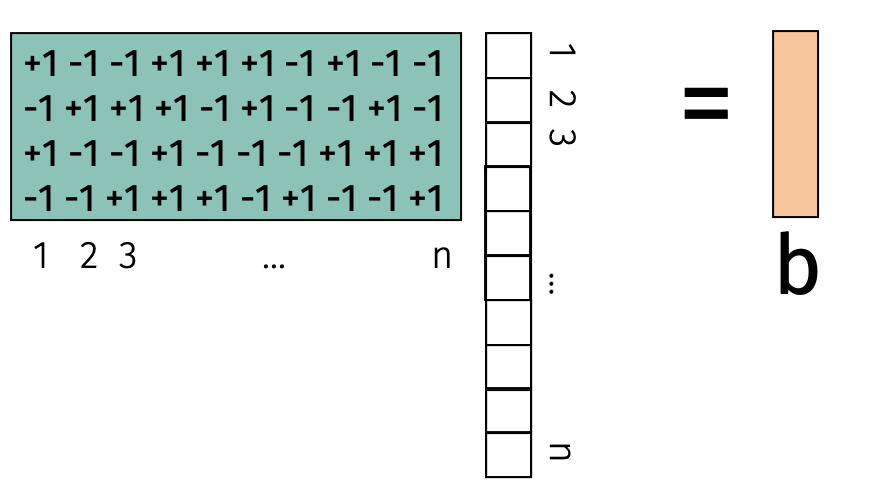
\includegraphics[width=.6\textwidth]{heavyhitters.png}
%	\end{center}
%	\begin{itemize}
%		\item Every time we receive a number $i$ in the stream, add column $\bv{A}_i$ to $\bv{b}$. 
%	\end{itemize}
%\end{frame}
%
%\begin{frame}
%	\frametitle{application: heavy hitters in data streams}
%	\begin{center}
%		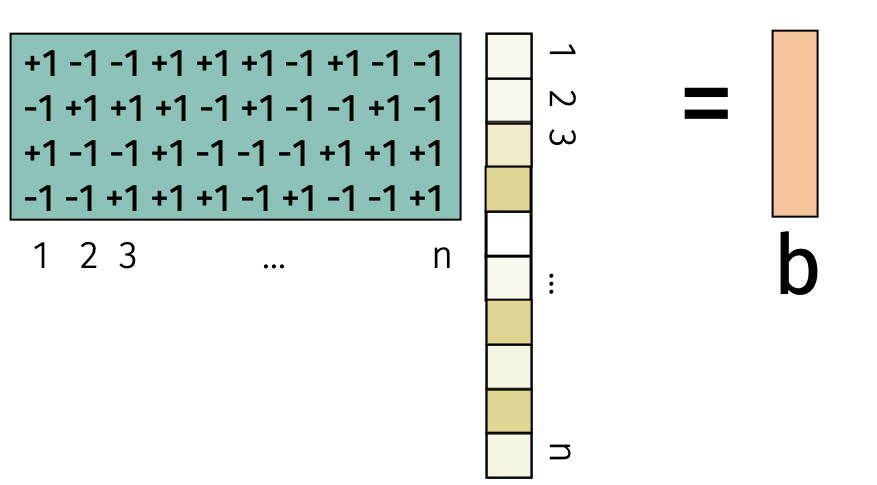
\includegraphics[width=.6\textwidth]{heavyhitterssparse.png}
%	\end{center}
%	\begin{itemize}
%		\item At the end $\bv{b} = \bv{A}\bv{x}$ for an approximately sparse $\bv{x}$ if there were only a few ``heavy hitters''. Recover $\bv{x}$ from $\bv{b}$ using a sparse recovery method (like $\ell_0$ minimization). 
%	\end{itemize}
%\end{frame}
%
%\begin{frame}
%	\frametitle{application: heavy hitters in data streams}
%	\begin{center}
%		\textbf{In contrast to the standard implementations of CountMin and related methods, sparse recovery based methods naturally handles both insertions or deletions.}
%	\end{center}
%	\begin{align*}
%		insert(4), insert(18), remove(4), insert(1), insert(2), remove(2)\ldots
%	\end{align*}
%	E.g. Amazon is monitoring what products people add to their ``wishlist'' and wants a list of most tagged products. Wishlists can be changed over time, including by removing items.
%\end{frame}
%
%



% \begin{frame}
% 	\frametitle{restricted isometry property}
% 	\begin{definition}[$(q,\epsilon)$-Restricted Isometry Property]
% 		A matrix $\bv{A}$ satisfies $(q,\epsilon)$-RIP if, for all $\bv{x}$ with $\|\bv{x}\|_0 \leq q$, 
% 		\begin{align*}
% 			(1-\epsilon)\|\bv{x}\|_2^2 \leq \|\bv{A}\bv{x}\|_2^2 \leq  (1+\epsilon)\|\bv{x}\|_2^2.
% 		\end{align*}
% 	\end{definition}
	
% 	Lots of other random matrices satisfy RIP as well. 
	
% 	One major theoretical question is if we can \emph{deterministically construct} good RIP matrices. Interestingly, if we want $(O(k),O(1))$ RIP, we can only do so with $O(k^2)$ rows (now very slightly better -- thanks to Bourgain et al.). 
	
% 	Whether or not a linear dependence on $k$ is possible with a deterministic construction is unknown.
% \end{frame}

% \begin{frame}[t]
% 	\frametitle{faster sparse recovery}
% 	\begin{theorem}[$\ell_0$-minimization]
% 		Suppose we are given $\bv{A} \in \R^{m\times n}$ and $\bv{b} = \bv{A}\bv{x}$ for an unknown $k$-sparse $\bv{x}$.
% 		If $\bv{A}$ is $(2k,\epsilon)$-RIP for any $\epsilon < 1$ then $\bv{x}$ is the unique minimizer of:
% 		\begin{align*}
% 			\min &\|\bv{z}\|_0 & &\text{subject to} & \bv{A}\bv{z} &= \bv{b} .
% 		\end{align*}
% 	\end{theorem}
% 	\begin{center}
% 		\textbf{Algorithm question:} Can we recover $\bv{x}$ using a faster method? Ideally in polynomial time.
% 	\end{center}
% \end{frame}

% \begin{frame}[t]
% 	\frametitle{basis pursuit}
% 	\textbf{Convex relaxation of the $\ell_0$ minimization problem:}
% 	\begin{problem}[Basis Pursuit, i.e. $\ell_1$ minimization.]
% 		\begin{align*}
% 			\min_{\bv{z}} &\|\bv{z}\|_1 & &\text{subject to} & \bv{Az} &= \bv{b} .
% 		\end{align*}
% 	\end{problem}
% 	\begin{itemize}
% 		\item Objective is convex. \vspace{2em}
		
% 		\item Optimizing over convex set.
% 	\end{itemize}
	
% 	\begin{center}
% 		\alert{What is one method we know for solving this problem?}
% 	\end{center}
% \end{frame}

% \begin{frame}[t]
% 	\frametitle{basis pursuit linear program}
% 	\textbf{Equivalent formulation:}
% 	\begin{problem}[Basis Pursuit Linear Program.]
% 		\begin{align*}
% 			\min_{\bv{w},\bv{z}}\, & \bv{1}^T\bv{w} & &\text{subject to} & \bv{Az} &= \bv{b}, \bv{w} \geq 0, -\bv{w} \leq \bv{z} \leq \bv{w}.
% 		\end{align*}
% 	\end{problem}
% 	Can be solved using any algorithm for linear programming. An Interior Point Method will run in $\sim O(n^{3.5})$ time.
% \end{frame}

% 	\begin{frame}[t]
% 	\frametitle{basis pursuit analysis}
% 	\begin{theorem}
% 		If $\bv{A}$ is $(3k, \epsilon)$-RIP for $\epsilon < .17$ and $\|\bv{x}\|_0 = k$, then $\bv{x}$ is the unique optimal solution of the Basis Pursuit LP).
% 	\end{theorem}
% 	\textbf{Two surprising things about this result:}
% 	\begin{itemize}
% 		\item Exponentially improve computational complexity with only a \emph{constant factor} overhead in measurement complexity.
% 		\item Typical ``relax-and-round'' algorithm, but rounding is not even necessary! Just return the solution of the relaxed problem. 
% 	\end{itemize}
% \end{frame}

% \begin{frame}[t]
% 	\frametitle{basis pursuit intuition}
% 	Suppose $\bv{A}$ is $2\times 1$, so $\bv{b}$ is just a scalar and $\bv{x}$ is a 2-dimensional vector.
% 	\begin{figure}[h]
% 		\centering
% 		\begin{subfigure}[t]{0.48\textwidth}
% 			\centering
% 			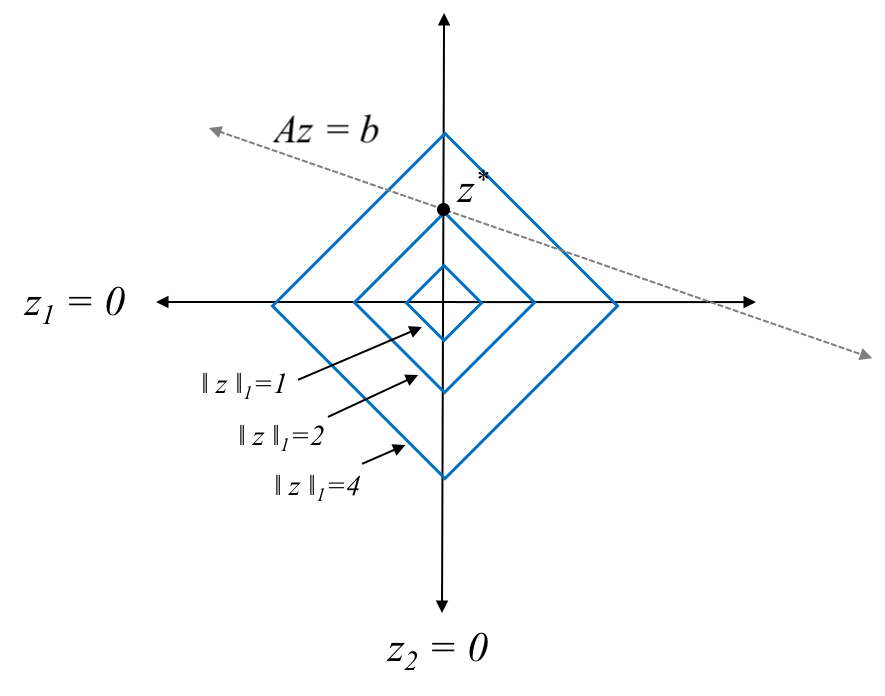
\includegraphics[width=\textwidth]{l1opt.png}
% 			\caption{Vertices of level sets of $\ell_1$ norm correspond to sparse solutions.}
% 		\end{subfigure}
% 		~
% 		\begin{subfigure}[t]{0.48\textwidth}
% 			\centering
% 			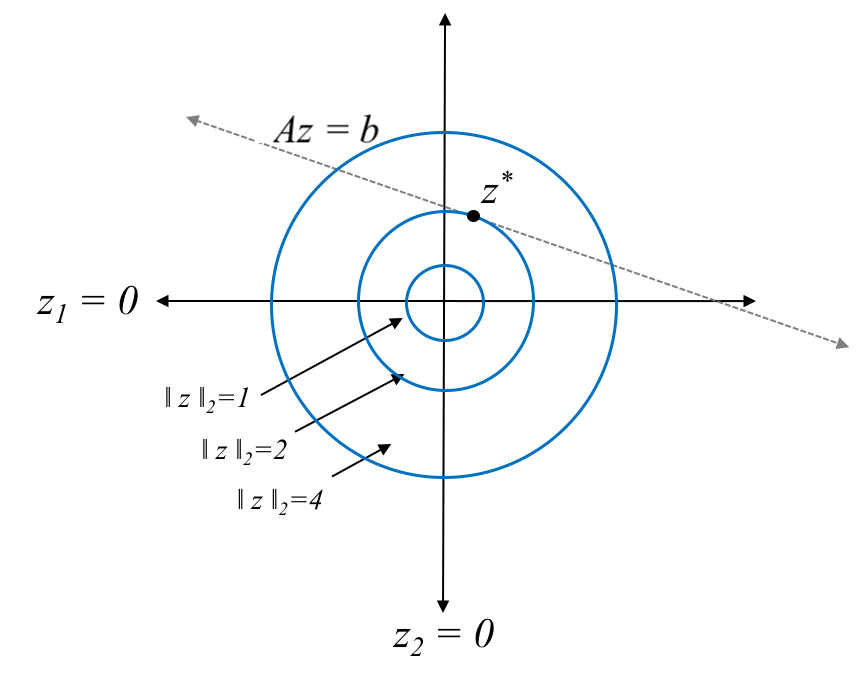
\includegraphics[width=\textwidth]{l2opt.png}
% 			\caption{This is not the case e.g. for the $\ell_2$ norm.}
% 		\end{subfigure}
% 	\end{figure}
% \end{frame}

% \begin{frame}[t]
% 	\frametitle{basis pursuit analysis}
% 	\begin{theorem}
% 		If $\bv{A}$ is $(3k, \epsilon)$-RIP for $\epsilon < .17$ and $\|\bv{x}\|_0 = k$, then $\bv{x}$ is the unique optimal solution of the Basis Pursuit LP).
% 	\end{theorem}
% 	\text{Similar proof to $\ell_0$ minimization:}
% 	\begin{itemize}
% 		\item By way of contradiction, assume $\bv{x}$ is \emph{not the optimal solution}. Then there exists some non-zero ${\Delta}$ such that:
% 		\begin{itemize}
% 			\item $\|\bv{x} + {\Delta}\|_1 \leq \|\bv{x}\|_1$
% 			\item $\bv{A}(\bv{x} + {\Delta}) = \bv{A}\bv{x}$. I.e. $\bv{A}{\Delta} = 0$.
% 		\end{itemize}
% 	\end{itemize}
% 	Difference is that we can no longer assume that $\Delta$ is sparse. 
	
% 	\begin{center}
% 		\alert{We will argue that $\Delta$ is approximately sparse.} 
% 	\end{center}
% \end{frame}

% \begin{frame}[t]
% 	\frametitle{tools needed}		
% 	\textbf{First tool:}
% 	\begin{align*}
% 		\text{For any $q$-sparse vector } &\bv{w}, & \|\bv{w} \|_2 \leq \|\bv{w} \|_1 \leq \sqrt{q}\|\bv{w}\|_2
% 	\end{align*}
% 	\vspace{3em}
	
% 	\textbf{Second tool:}
% 	\begin{align*}
% 		\text{For any norm and vectors $\bv{a},\bv{b}$, }& & \|\bv{a}+ \bv{b}\| \geq \|\bv{a}\| - \|\bv{b}\|
% 	\end{align*}
	
	
% \end{frame}

% \begin{frame}[t]
% 	\frametitle{basis pursuit analysis}
% 	\textbf{Some definitions:}
% 	\begin{center}
% 		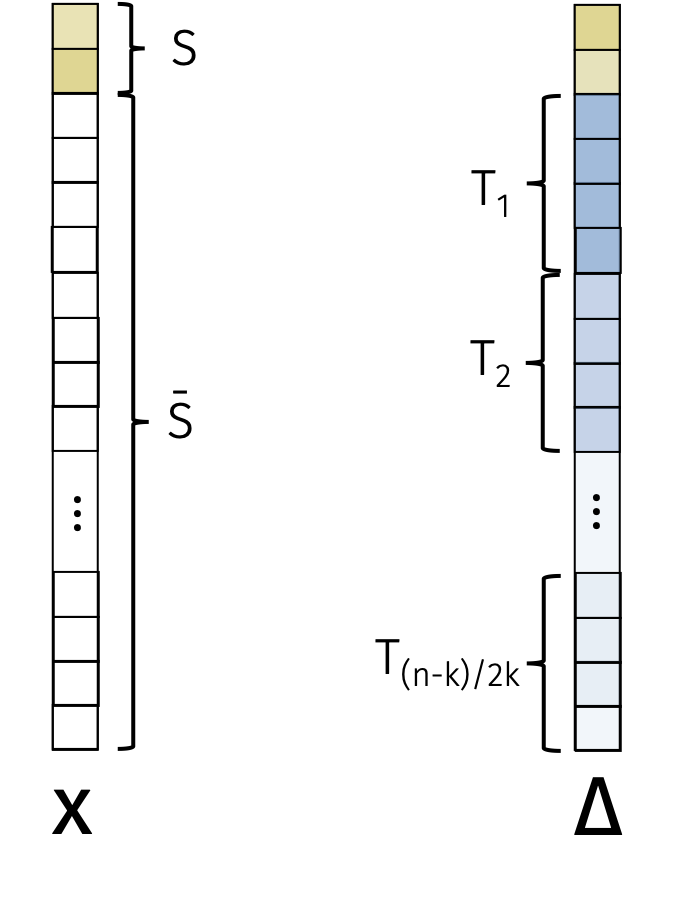
\includegraphics[width=.5\textwidth]{indexingForProof.png}
% 	\end{center}
% 	$T_1$ contains the $2k$ indices with largest value in $\Delta$ \emph{that are zero in $\bv{x}$}. $T_2$ contains the next $2k$ largest entries, etc. 
% \end{frame}

% \begin{frame}[t]
% 	\frametitle{basis pursuit analysis}
% 	\textbf{Claim 1:}
% 	$\|\Delta_{S}\|_1 \geq \|\Delta_{\bar{S}}\|_1$
% \end{frame}

% \begin{frame}[t]
% 	\frametitle{basis pursuit analysis}
% 	\textbf{Claim 2:}
% 	$\|\Delta_{S}\|_2 \geq \sqrt{2}\sum_{j\geq 2} \|\bs{\Delta}_{T_j}\|_2$:
	
% 	\begin{align*}
% 		\|\bs{\Delta}_s\|_2 \geq \frac{1}{\sqrt{k}} \|\bs{\Delta}_{S}\|_1 \geq \frac{1}{\sqrt{k}}\|\bs{\Delta}_{\bar{S}}\|_1 = \frac{1}{\sqrt{k}}\sum_{j\geq 1} \|\bs{\Delta}_{T_j}\|_1.
% 	\end{align*}
	
% 	Claim: $\|\bs{\Delta}_{T_j}\|_1 \geq \sqrt{2k}\|\bs{\Delta}_{T_{j+1}}\|_2$
% \end{frame}

% \begin{frame}[t]
% 	\frametitle{basis pursuit analysis}
% 	\textbf{Finish up proof by contradiction:}
% 	Recall that $\bv{A}$ is assumed to have the $(3k,\epsilon)$ RIP property.
	
% 	\begin{align*}
% 		0 = \|\bv{A}\bs{\Delta}\|_2 \geq  \|\bv{A}\bs{\Delta}_{S\cup T_1}\|_2 - \sum_{j\geq 2} \|\bv{A}\bs{\Delta}_{T_j}\|_2
% 	\end{align*}
% \end{frame}

% \begin{frame}
% 	\frametitle{faster methods}
% 	A lot of interest in developing even faster algorithms that avoid using the ``heavy hammer'' of linear programming and run in even faster than $O(n^{3.5})$ time. 
	
% 	\begin{itemize}
% 		\item \textbf{Iterative Hard Thresholding}: Looks a lot like projected gradient descent. Solve $\min_{\bv{z}} \|\bv{Az} - \bv{b}\|$ with gradient descent while continually projecting $z$ back to the set of $k$-sparse vectors. Runs in time \alert{$\sim O(n k\log n)$} for Gaussian measurement matrices and \alert{$O(n\log n)$} for subsampled Fourer matrices.
% 		\item Other ``first order'' type methods: Orthogonal Matching Pursuit, CoSaMP, Subspace Pursuit, etc.
% 	\end{itemize}
	
% 	%	One example of such an algorithm is Iterative Hard Thresholding \cite{iht}, which looks a lot like the projected gradient descent method we saw in class. The idea is to solve $\min_z \|z - Ax\|$ via a gradient method, . While this set is \emph{not convex} it's possible to show that the method still converges very rapidly. See \url{http://people.seas.harvard.edu/~minilek/cs229r/fall13/lec/lec18.pdf} for an analysis. The runtime of the method is approximately $O(n k\log n)$ for Gaussian measurement matrices and $O(n\log n)$ for subsampled Fourier matrices. Other ``first order'' type methods obtain similar running times. If you are interested in learning more, some algorithms to look up include ``Orthogonal Matching Pursuit'', "CoSaMP", and ``Subspace Pursuit''.
% \end{frame}

% \begin{frame}
% 	\frametitle{faster methods}
% 	When $\bv{A}$ is a subsampled Fourier matrix, there are now methods that run in \alert{\emph{$O(k\log^c n)$}} time [Hassanieh, Indyk, Kapralov, Katabi, Price, Shi, etc. 2012+].
	
% 	\begin{center}
% 		\textbf{Hold up...}
% 	\end{center}
	
% \end{frame}

% \begin{frame}
% 	\frametitle{sparse fourier transform}
% 	\textbf{Corollary:} When $\bv{x}$ is $k$-sparse, we can compute the inverse Fourier transform $\bv{F}^*\bv{F}\bv{x}$ of $\bv{F}\bv{x}$ in $O(k\log^c n)$ time!
% 	\begin{itemize}
% 		\item Randomly subsample $\bv{F}\bv{x}$.
% 		\item Feed that input into our sparse recovery algorithm to extract $\bv{x}$. 
% 	\end{itemize}
% 	\begin{center}
% 		\alert{Fourier and inverse Fourier transforms in \emph{sublinear time} when the output is sparse. }
		
% 		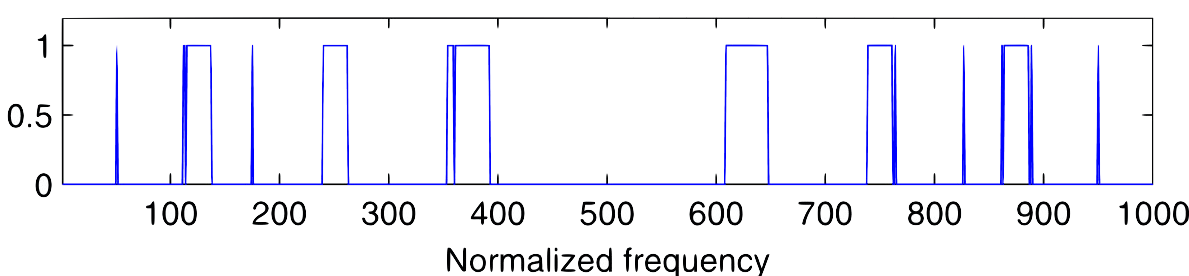
\includegraphics[width=.8\textwidth]{multiband.png}
% 	\end{center}
% 	\textbf{Applications in:} Wireless communications, GPS, protein imaging, radio astronomy, etc. etc. 
% \end{frame}

% \begin{frame}
% 	\frametitle{compressed sensing from generative models}
% 	\begin{center}
% 		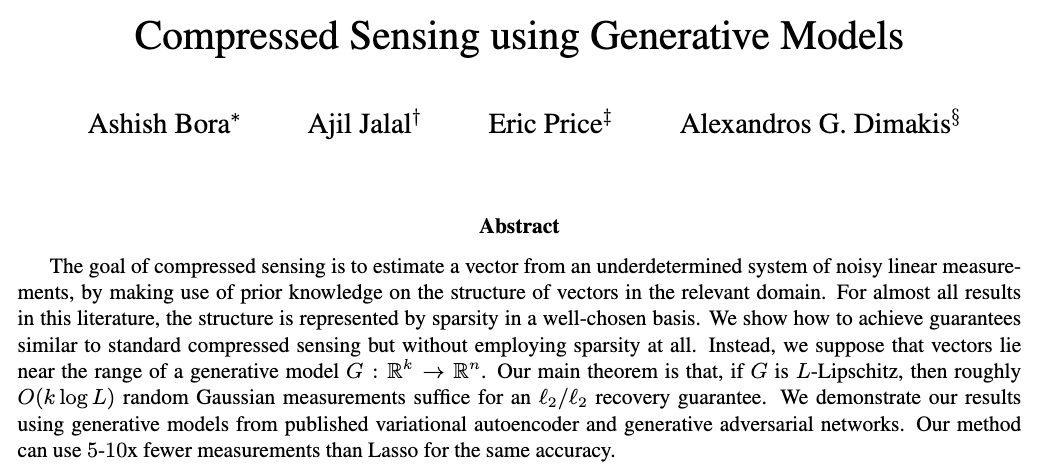
\includegraphics[width=.7\textwidth]{price1.png}
		
% 		\vspace{.5em}
% 				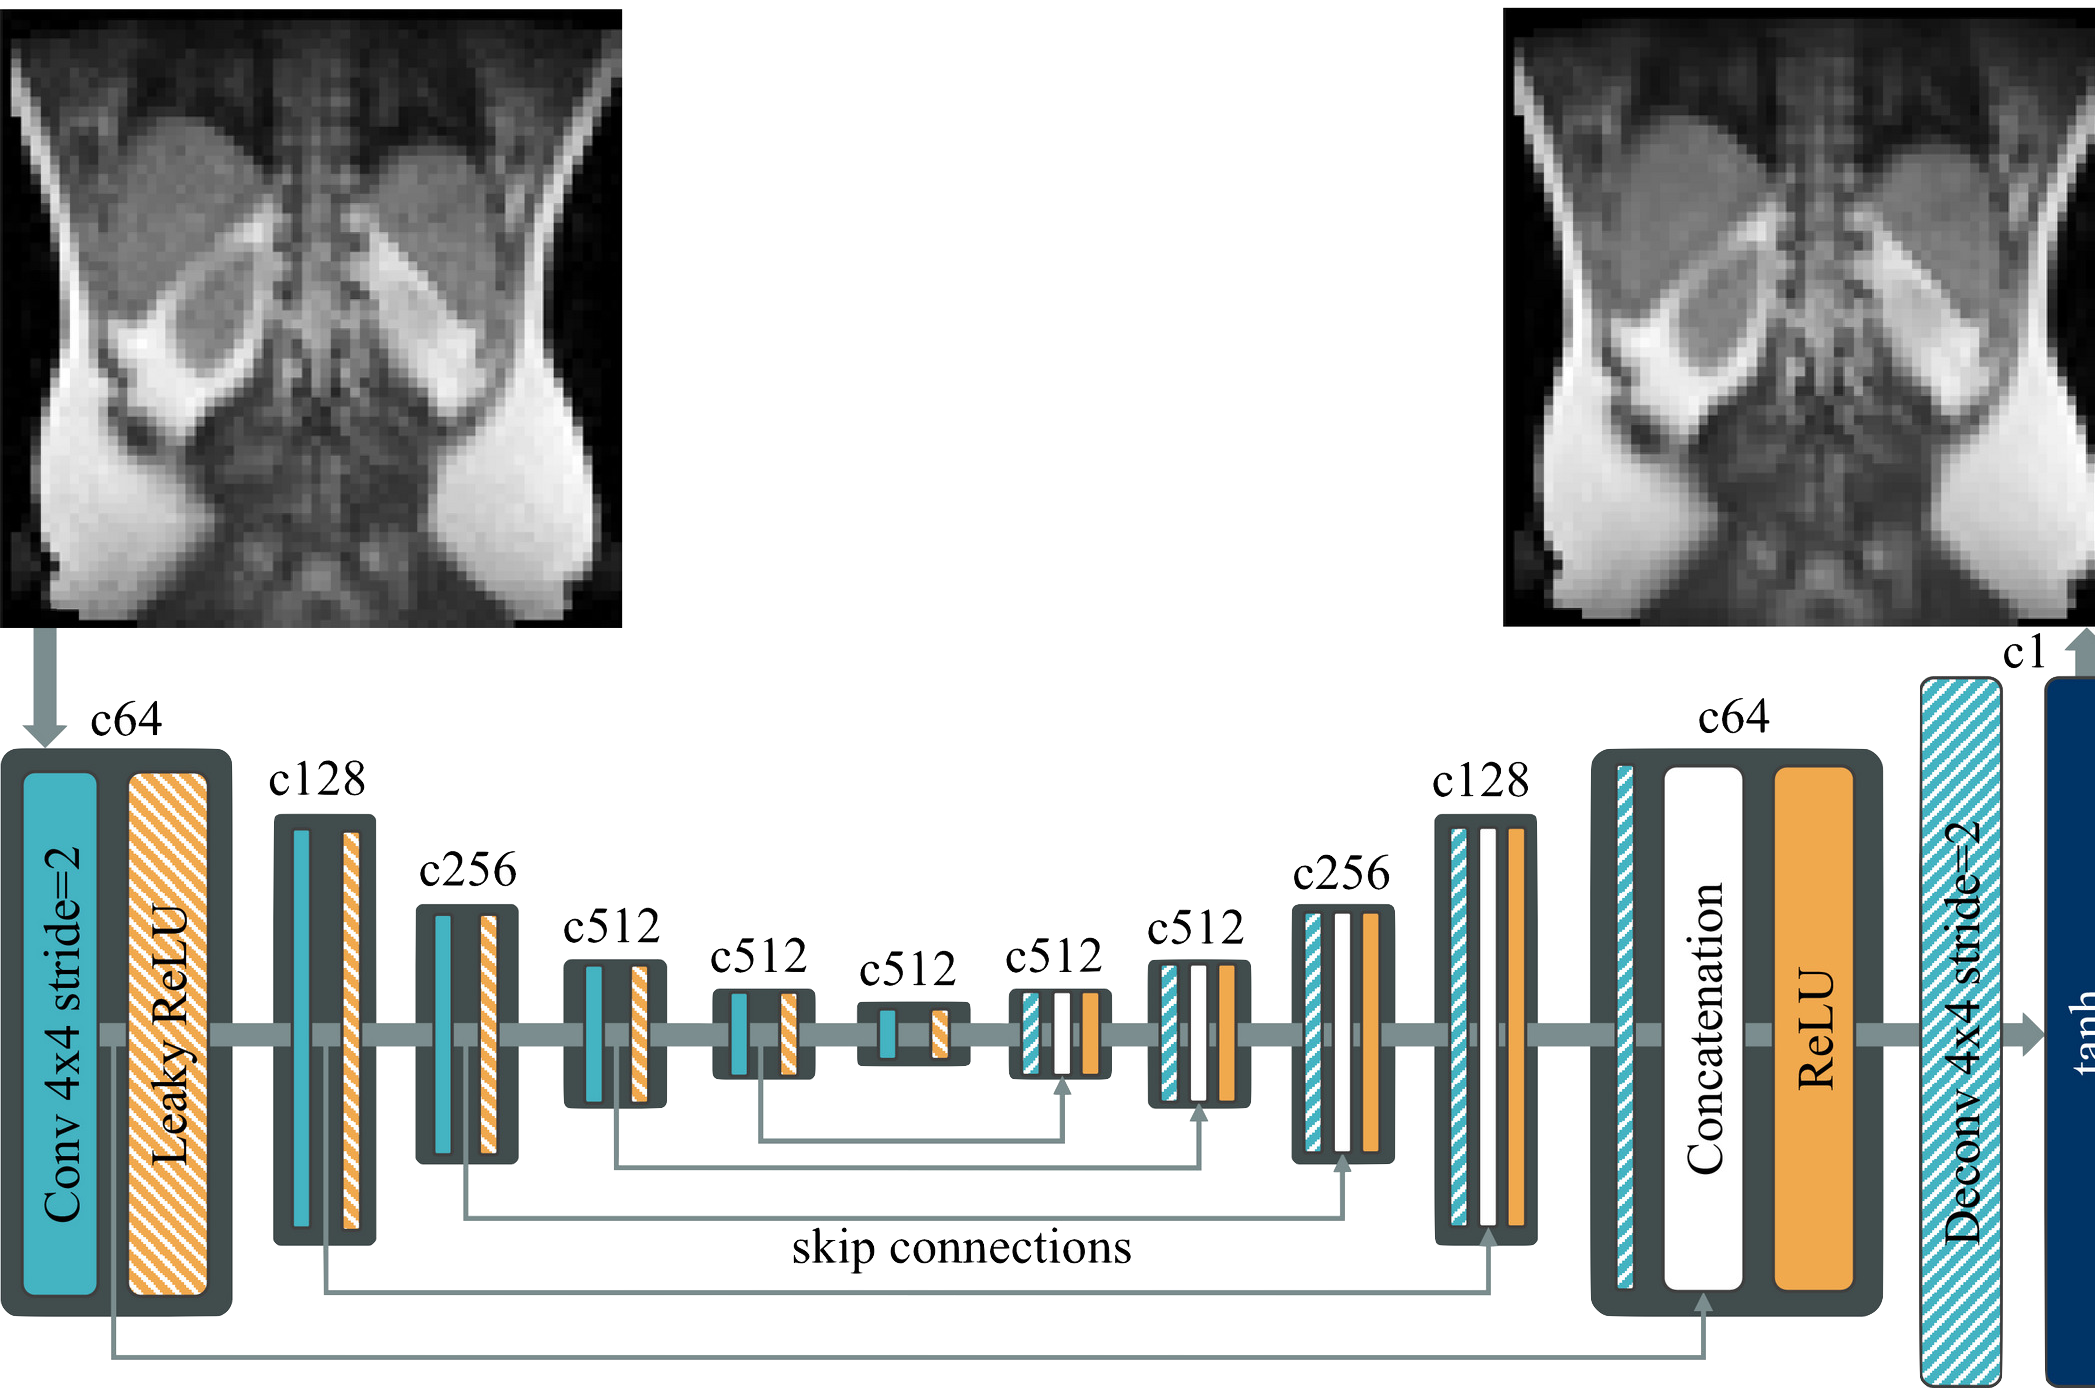
\includegraphics[width=.5\textwidth]{medical_autoencode.png}
% 	\end{center}
% \end{frame}

% \begin{frame}
% 	\frametitle{compressed sensing from generative models}
% 	\begin{center}
% 		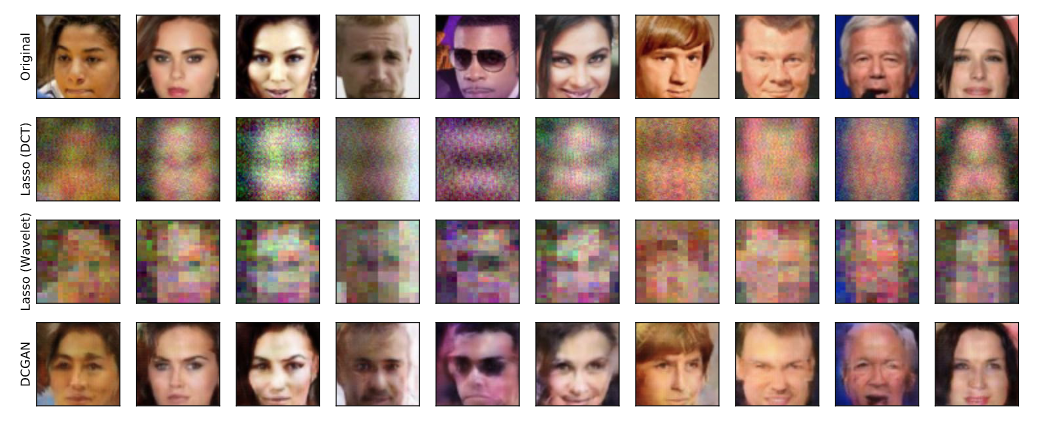
\includegraphics[width=.9\textwidth]{price2.png}
% 	\end{center}
	
% \end{frame}

\end{document} 




